%%%%%%%%%%%%%%%%%%%%%%%%%%%%%%%%%%%%%%%%%%%%%%%%%%%%%%%%%%%%%%%%%%%%%%%%%%%%%%%%%%%%%%
% To make formatting easy tell LaTeX what kind of document you want to write
% by changing the according {} to {#1}
%%%%%%%%%%%%%%%%%%%%%%%%%%%%%%%%%%%%%%%%%%%%%%%%%%%%%%%%%%%%%%%%%%%%%%%%%%%%%%%%%%%%%%
%
% Most of the choices and things that need to be adjusted are maked 
% with a commented "TODO". Adjust the given value the one correct your your case.
%
%%%%%%%%%%%%%%%%%%%%%%%%%%%%%%%%%%%%%%%%%%%%%%%%%%%%%%%%%%%%%%%%%%%%%%%%%%%%%%%%%%%%%%

% Dissertation
\newcommand{\Diss}[1]{}
% Diplomarbeit
\newcommand{\Dipl}[1]{}
% Master Thesis
\newcommand{\MS}[1]{#1}
% Studienarbeit
\newcommand{\Stud}[1]{}

\newcommand{\BachelorT}[1]{} %%TODO: mark the corret one with a #1

%%%%%%%%%%%%%%%%%%%%%%%%%%%%%%%%%%%%%%%%%%%%%%%%%%%%%%%%%%%%%%%%%%%%%%%%%%%%%%%%%%%%%%
% Which language do you want to write in
%%%%%%%%%%%%%%%%%%%%%%%%%%%%%%%%%%%%%%%%%%%%%%%%%%%%%%%%%%%%%%%%%%%%%%%%%%%%%%%%%%%%%%
%English
\newcommand{\EN}[1]{#1} %%TODO: Choose the correct language
%German
\newcommand{\DE}[1]{}

%%%%%%%%%%%%%%%%%%%%%%%%%%%%%%%%%%%%%%%%%%%%%%%%%%%%%%%%%%%%%%%%%%%%%%%%%%%%%%%%%%%%%%
% For print single or double page?
%%%%%%%%%%%%%%%%%%%%%%%%%%%%%%%%%%%%%%%%%%%%%%%%%%%%%%%%%%%%%%%%%%%%%%%%%%%%%%%%%%%%%%
\newcommand{\single}[1]{#1} %%TODO: Choose
\newcommand{\double}[1]{}

%%%%%%%%%%%%%%%%%%%%%%%%%%%%%%%%%%%%%%%%%%%%%%%%%%%%%%%%%%%%%%%%%%%%%%%%%%%%%%%%%%%%%%
% Now this is followed by a lot of page and command definitions. For the beginning you 
% should be able to continue where you find the next comment section like this one.
% However, you might want to take a look a the definitions sometime to be able to use 
% them. Of course you can also add the defintions you needed yourself.
%%%%%%%%%%%%%%%%%%%%%%%%%%%%%%%%%%%%%%%%%%%%%%%%%%%%%%%%%%%%%%%%%%%%%%%%%%%%%%%%%%%%%%

\single{\documentclass[12pt,a4paper,oneside,german,english]{book}}
\double{\documentclass[12pt,a4paper,twoside,german,english]{book}}
\usepackage[normalem]{ulem}
\usepackage[ngerman,main=english]{babel}
%\usepackage[draft,breaklinks=true,colorlinks=false,dvips,bookmarks,pdffitwindow,pdfcenterwindow=true,pdfstartview=Fit]{hyperref}
%\usepackage[breaklinks=true,colorlinks=false,dvips,bookmarks,pdffitwindow,pdfcenterwindow=true,pdfstartview=Fit]{hyperref}
\usepackage{setspace}
\usepackage{cite}
\usepackage{float,times} 
\usepackage[utf8x]{inputenc}
\usepackage[T1]{fontenc}
\usepackage{amsmath,amsthm,latexsym,amssymb}
\usepackage[dvips]{epsfig}
% \usepackage{subfigure}
\usepackage{rotating}

\usepackage{graphicx}
\usepackage{subcaption}

%\usepackage[outputdir=obj/]{minted} %% Use for advanced build mechanic, needs newest minted style file
%\usepackage{minted} %% use for fancy syntax highlighting of code. Needs "pygmetize" and the minted style file
\usepackage{xspace}

\usepackage{xcolor}
\usepackage{afterpage}
\usepackage{multirow}
\usepackage{array}

\usepackage{pdfpages}

\usepackage{booktabs}% http://ctan.org/pkg/booktabs
\newcommand{\tabitem}{~~\llap{\textbullet}~~}

\usepackage{capt-of}
\usepackage{caption}
\usepackage{listings}
% \renewcommand{\lstlistingname}{Quelltext}
\renewcommand*{\lstlistlistingname}{List of \lstlistingname s}
%\usepackage[german]{fancyref}
\usepackage[english]{fancyref}
\newcommand*{\fancyreflstlabelprefix}{lst}
\newcommand*{\fancyrefitelabelprefix}{ite}
\newcommand*{\fancyrefparlabelprefix}{par}

\fancyrefaddcaptions{german}{
  \providecommand*{\freflstname}{Listing}
  \providecommand*{\Freflstname}{Listing}
}

\frefformat{plain}{\fancyreflstlabelprefix}{\freflstname\fancyrefdefaultspacing#1}
\Frefformat{plain}{\fancyreflstlabelprefix}{\Freflstname\fancyrefdefaultspacing#1}

\frefformat{plain}{\fancyreflstlabelprefix}{
  \freflstname\fancyrefdefaultspacing#1#3
}
\Frefformat{plain}{\fancyreflstlabelprefix}{
  \Freflstname\fancyrefdefaultspacing#1#3
}

\fancyrefaddcaptions{german}{
  \providecommand*{\frefitename}{Liste}
  \providecommand*{\Frefitename}{Liste}
}

\frefformat{plain}{\fancyrefitelabelprefix}{\frefitename\fancyrefdefaultspacing#1}
\Frefformat{plain}{\fancyrefitelabelprefix}{\Frefitename\fancyrefdefaultspacing#1}

\frefformat{plain}{\fancyrefitelabelprefix}{
  \frefitename\fancyrefdefaultspacing#1#3
}
\Frefformat{plain}{\fancyrefitelabelprefix}{
  \Frefitename\fancyrefdefaultspacing#1#3
}

\fancyrefaddcaptions{german}{
  \providecommand*{\frefparname}{Paragraph}
  \providecommand*{\Frefparname}{Paragraph}
}

\frefformat{plain}{\fancyrefparlabelprefix}{\frefparname\fancyrefdefaultspacing#1}
\Frefformat{plain}{\fancyrefparlabelprefix}{\Frefparname\fancyrefdefaultspacing#1}

\frefformat{plain}{\fancyrefparlabelprefix}{
  \frefparname\fancyrefdefaultspacing#1#3
}
\Frefformat{plain}{\fancyrefparlabelprefix}{
  \Frefparname\fancyrefdefaultspacing#1#3
}

\renewcommand{\fancyrefdefaultformat}{plain}

\newcommand{\ThesisTitle}{Property Generation for Pipelined Processors in a Property-Driven Design Approach} %%TODO
\newcommand{\ThesisTitleGerman}{Hier Deutschen Titel Einf\"ugen} %%TODO %NOTE: for some reason, LaTeX does not understand utf8 here...

% format page layout.

%\setlength{\topmargin}{0cm}
%\setlength{\textwidth}{15cm}
%\setlength{\textheight}{22cm}
%\setlength{\oddsidemargin}{1cm}
%\setlength{\evensidemargin}{0cm}
\setlength{\headheight}{15pt}

\setlength{\emergencystretch}{1em}

\setlength{\voffset}{-0cm}
\setlength{\topmargin}{0cm}
\setlength{\headheight}{0.54cm}
\setlength{\textheight}{23cm}
% \setlength{\headsep}{1.5cm}
% \setlength{\hoffset}{-2.54cm}
\setlength{\hoffset}{0cm}
\setlength{\oddsidemargin}{0.46cm}
\setlength{\evensidemargin}{0.46cm}
\setlength{\textwidth}{16cm}
\setlength{\marginparsep}{0cm}
\setlength{\marginparwidth}{1.54cm}

% adjust linespacing
\linespread{1.3}

\usepackage{parskip}
% \setlength{\footskip}{1cm}
% \setlength{\parindent}{0cm}
 \setlength{\parskip}{1em}

\setcounter{secnumdepth}{3}
\setcounter{tocdepth}{1}

\usepackage{fancyhdr}
\pagestyle{fancy}
\fancyhead{} % clear all header fields
\double{\fancyhead[LE]{\slshape \nouppercase{\leftmark}}} % chapter titles
\fancyhead[RO]{\slshape \nouppercase{\rightmark}} % section titles
\fancyfoot{} % clear all footer fields
\fancyfoot[C]{\thepage}


\usepackage[%dvips,
	colorlinks=false,
	bookmarks,
	pdffitwindow,
	pdfcenterwindow=true,
	pdfstartview=Fitpdftex,
	pdfauthor={Insert Author Name here}, %%TODO
% 	pdftitle={\EN{\ThesisTitle}\DE{\ThesisTitleGerman}},
	pdftitle={\EN{\ThesisTitle}},
	pdfsubject={}, % one sentence summery %%TODO
	pdfkeywords={Thesis,Hardware,Simulation,System-Modelling}, %TODO: comma-seperated keywords
	pdfproducer={Latex with hyperref},
	pdfcreator={}]{hyperref}

%%%%%%%%%%%%%%%%%%%%%%%%%%%%%%%%%%%%%%%%%%%%%%%%%%%
% Overly fancy comments
%%%%%%%%%%%%%%%%%%%%%%%%%%%%%%%%%%%%%%%%%%%%%%%%%%%
%% uncomment the ifthen block if the enhanched build mechanic is used
% \providecommand\printcomments{false}
% \usepackage{ifthen}
% \ifthenelse{ \equal{\printcomments}{true} }{
\newcommand{\comment}[3]{\marginpar{\textcolor{#2}{Comment: #1}}\textcolor{#2}{\textit{[#1: #3]}}}
\newcommand{\SupervisorComment}[1]{\comment{Supervisor}{red}{#1}} %%TODO: exchange "SupervisorComment" and "Supervisor" with initials
\newcommand{\StudentComment}[1]{\comment{Student}{blue}{#1}} %%TODO: exchange "StudentComment" and "Student" with initials
% }{
% \newcommand{\TF}[1]{}
% \newcommand{\LA}[1]{}
% }
%%%%%%%%%%%%%%%%%%%%%%%%%%%%%%%%%%%%%%%%%%%%%%%%%%%
%\usepackage{showframe}

\usepackage[shortlabels]{enumitem}


\definecolor{codegreen}{rgb}{0,0.6,0}
\definecolor{codegray}{rgb}{0.5,0.5,0.5}
\definecolor{codepurple}{rgb}{0.58,0,0.82}
\definecolor{backcolour}{rgb}{1,1,1}

\lstdefinestyle{mystyle}{
    backgroundcolor=\color{backcolour},   
    commentstyle=\color{codegreen},
    keywordstyle=\color{blue},
    numberstyle=\tiny\color{codegray},
    stringstyle=\color{codepurple},
    basicstyle=\ttfamily\footnotesize,
    breakatwhitespace=false,         
    breaklines=true,                 
    captionpos=b,                    
    keepspaces=true,                 
    numbers=left,                    
    numbersep=3pt,                  
    showspaces=false,                
    showstringspaces=false,
    showtabs=false,                  
    tabsize=2
}

\lstset{style=mystyle}

\newcommand{\SSQED }{S$^2$QED}

%%%%%%%%%%%%%%%%%%%%%%%%%%%%%%%%%%%%%%%%%%%%%%%%%%%%%%%%%%%%%%%%%%%%%%%%%%%%%%
% 
%  Some useful definitions 
% 
%%%%%%%%%%%%%%%%%%%%%%%%%%%%%%%%%%%%%%%%%%%%%%%%%%%%%%%%%%%%%%%%%%%%%%%%%%%%%%


\newcommand{\refsec}[1]{Sec.~\ref{sec:#1}}
\newcommand{\reffig}[1]{Fig.~\ref{fig:#1}}
\newcommand{\reftab}[1]{Tab.~\ref{tab:#1}}
\newcommand{\refalg}[1]{Alg.~\ref{alg:#1}}
\newcommand{\refdef}[1]{Def.~\ref{def:#1}}

\newcommand{\URLFORMAT}[1]{\mbox{\sffamily\small #1}}

\newcommand{\CODESYMBOL}[1]{\textsf{\textit{\small #1}}}

\newcommand{\CTLOPERATOR}[1]{\mbox{\textsf{\textup{#1}}}}
\newcommand{\CTLAX}{\CTLOPERATOR{AX}}
\newcommand{\CTLAF}{\CTLOPERATOR{AF}}
\newcommand{\CTLAG}{\CTLOPERATOR{AG}}
\newcommand{\CTLEX}{\CTLOPERATOR{EX}}
\newcommand{\CTLEF}{\CTLOPERATOR{EF}}
\newcommand{\CTLEG}{\CTLOPERATOR{EG}}
\newcommand{\LTLX}{\CTLOPERATOR{X}}
\newcommand{\LTLXT}[1]{\mbox{$\CTLOPERATOR{X}^{#1}$}}
\newcommand{\LTLF}{\CTLOPERATOR{F}}
\newcommand{\LTLG}{\CTLOPERATOR{G}}
\newcommand{\LTLU}{\CTLOPERATOR{U}}
\newcommand{\LTLR}{\CTLOPERATOR{R}}
\newcommand{\LTLW}{\CTLOPERATOR{W}}

\newcommand{\LTLS}{\CTLOPERATOR{S}}



%%%%%%%%%%%%%%%%%%%%%%%%%%%%%%%%%%%%%%%%%%%%%%%%%%%%%%%%%%%%%%%%%%%%%%%%%%%%%%
% For revisions: 
\definecolor{newtextcolor}{rgb}{0,0,0.5}
\newenvironment{newtext}{\color{newtextcolor}}{}
\definecolor{oldtextcolor}{rgb}{0.4,0.4,0.4}
\newenvironment{oldtext}{\color{oldtextcolor}\par\textit{\sffamily Begin (old
    text)}\par}{\hfill\textit{\sffamily End (old text)}\par}
\newcommand{\textnew}[1]{{\color{newtextcolor}#1}}


%For code: 
\newcommand{\key}[1]{\textcolor{BlueViolet}{#1}}
\newcommand{\ckey}[1]{\textcolor{blue}{#1}}
\newcommand{\type}[1]{\textcolor{Green}{#1}}
\newcommand{\port}[1]{\textcolor{RedViolet}{#1}}
\newcommand{\macro}[1]{\textcolor{Sepia}{#1}}
\newcommand{\tend}{\key{t\_end}\textcolor{RedViolet}{(}length\textcolor{RedViolet}{)}~\textcolor{RedViolet}{\#\#}0~}
\newcommand{\tstart}{ \key{t} \textcolor{RedViolet}{\#\#}0~}

%ITL Properties:
\newcommand{\ITLKW}[1]{{\color{blue} #1}}
\newcommand{\ITLAT}[1]{\ITLKW{at t+{}#1: }}
\newcommand{\ITLOR}{\ITLKW{\textbar\,\textbar}}
\newcommand{\ITLENDL}{\ITLKW{;}}
\newcommand{\ITLPREV}{\ITLKW{prev}}
\definecolor{DARKGREEN}{RGB}{0,100,0}
\newcommand{\ITLCOMMENT}[1]{{\color{DARKGREEN}- - #1}}


%Text

\newcommand{\tsCODE}[1]{\textsf{\textit{\small #1}}}

%Environments
\newtheorem{definition}{Definition}
\newtheorem{theorem}{Theorem}

%Abbreviations:
\newcommand{\SYSTEMCPPA}{SystemC-PPA}
\newcommand{\NOP}{non-overlap pipelining}
\newcommand{\OP}{overlap pipelining}
\newcommand{\BP}{base property}
\newcommand{\RP}{relaxed property}
\newcommand{\PPDD}{PPDD}
\newcommand{\PDDTOOL}{DeSCAM} 
\newcommand{\SYMBOLNAME}[1]{\mbox{\textsf{\textsl{\small #1}}\,}}
\newcommand{\BOOLTRUE}{\SYMBOLNAME{true}} 
\newcommand{\BOOLFALSE}{\SYMBOLNAME{false}}

% symbols of PPA
\newcommand{\CONCAT}{\mbox{$\odot$}}
\newcommand{\IMPORTANT}{\mbox{$\Psi$}}
  % message predicate
\newcommand{\MSGPRED}{\mbox{$\mu$}}
  % operational input predicate
\newcommand{\INPPRED}{\mbox{$\iota$}}
  % trigger 
\newcommand{\TRIGPRED}{\mbox{$\iota$}}

  %operational path
\newcommand{\oppath}{\ensuremath\mbox{$\mathtt{opath}$}}
%\newcommand\oppath{\mathrel{\overset{\makebox[0pt]{\mbox{\normalfont\tiny\sffamily oper}}}{\pi}}}

  %operational output
%\newcommand{\opout}{\ensuremath\mbox{$\mathtt{oout}$}}

  %color similar symbol
\newcommand\colsim{\mathrel{\overset{\makebox[0pt]{\mbox{\normalfont\tiny\sffamily color}}}{=}}}

%state, input, output color
\newcommand{\nodecolor}{\ensuremath\mbox{$\mathtt{f_{C}}$}}
\newcommand{\statecolor}{\ensuremath\mbox{$\mathtt{f_{SC}}$}}
\newcommand{\incolor}{\ensuremath\mbox{$\mathtt{f_{XC}}$}}
\newcommand{\outcolor}{\ensuremath\mbox{$\mathtt{f_{YC}}$}}

\newcommand{\notimplies}{%
  \mathrel{{\ooalign{\hidewidth$\not\phantom{=}$\hidewidth\cr$\implies$}}}}


% PredCol
\newcommand{\statepredcolor}{\ensuremath\mbox{$\mathtt{B_{\eta{}C}}$}}
\newcommand{\inputpredcolor}{\ensuremath\mbox{$\mathtt{B_{\iota{}C}}$}}
\newcommand{\outputpredcolor}{\ensuremath\mbox{$\mathtt{B_{\mu{}C}}$}}
% ColPred
\newcommand{\statecolorpred}{\ensuremath\mbox{$\mathtt{B_{C\eta}}$}}
\newcommand{\inputcolorpred}{\ensuremath\mbox{$\mathtt{B_{C\iota}}$}}
\newcommand{\outputcolorpred}{\ensuremath\mbox{$\mathtt{B_{C\mu}}$}}


% text style for operators: 
\newcommand{\tsOPERATOR}[1]{\mbox{\textrm{\textup{#1}}}}

% IMG and other operators
\newcommand{\IMG}{\tsOPERATOR{img}} %image
\newcommand{\PRE}{\tsOPERATOR{pre}} %pre-image

\newcommand\LFP{\mathrel{\overset{\makebox[0pt]{\mbox{\normalfont\scriptsize\sffamily fp}}}{\mbox{\normalfont\footnotesize\sffamily <}}}}
\newcommand\GFP{\mathrel{\overset{\makebox[0pt]{\mbox{\normalfont\scriptsize\sffamily fp}}}{\mbox{\normalfont\footnotesize\sffamily >}}}}

\newcommand{\ISPATH}{\tsOPERATOR{ispath}}
\newcommand{\ISOPERATION}{\tsOPERATOR{isoperation}}
\newcommand{\ISOUTPUT}{\tsOPERATOR{isoutput}}
\newcommand{\INPUT}{\tsOPERATOR{input}}
\newcommand{\OUTPUT}{\tsOPERATOR{output}}
% \newcommand{\ANY}{\tsOPERATOR{any}}
\newcommand{\STUTTER}{\tsOPERATOR{stutter}}

% NEXT operator takes a subscript in math mode: 
\newcommand{\NEXT}[1]{\mbox{\tsOPERATOR{next}}_{#1}}


%%% Local Variables: 
%%% mode: latex
%%% TeX-master: "binder"
%%% End: 


%%%%%%%%%%%%%%%%%%%%%%%%%%%%%%%%%%%%%%%%%%%%%%%%%%%%%%%%%%%%%%%%%%%%%%%%%%%%%%
%  Collaborative editing in EIS group
%  
%  Let NN be your initials. 
%  The following macros are defined: 
%
%  \NNINS{a}     - Suggest inserting the text a. 
%  \NNDEL{a}     - Suggest deleting the text a. 
%  \NNREP{a}{b}  - Suggest replacing a by b. 
%  \NNSAY{a}     - Comment by saying a.
% 
%%%%%%%%%%%%%%%%%%%%%%%%%%%%%%%%%%%%%%%%%%%%%%%%%%%%%%%%%%%%%%%%%%%%%%%%%%%%%%


%%%%%%%%%%%%%%%%%%%%%%%%%%%%%%%%%%%%%%%%%%%%%%%%%%%%%%%%%%%%%%%%%%%%%%%%%%%%%%
%
%   Required packages:
% 
%   \usepackage{xcolor}
%   \usepackage{ifthen}
%   \usepackage[normalem]{ulem}
%
%   Place those in the file prefix.tex
%
%%%%%%%%%%%%%%%%%%%%%%%%%%%%%%%%%%%%%%%%%%%%%%%%%%%%%%%%%%%%%%%%%%%%%%%%%%%%%%


%%%%%%%%%%%%%%%%%%%%%%%%%%%%%%%%%%%%%%%%%%%%%%%%%%%%%%%%%%%%%%%%%%%%%%%%%%%%%%
% MARKUP switch
% Set to true if markup is to be shown, false otherwise

\newboolean{MARKUP}
\setboolean{MARKUP}{true}
% \setboolean{MARKUP}{false}

%
%%%%%%%%%%%%%%%%%%%%%%%%%%%%%%%%%%%%%%%%%%%%%%%%%%%%%%%%%%%%%%%%%%%%%%%%%%%%%%

%%%%%%%%%%%%%%%%%%%%%%%%%%%%%%%%%%%%%%%%%%%%%%%%%%%%%%%%%%%%%%%%%%%%%%%%%%%%%%
%
%  Authors

%  Every author can have their own distinctive markup color. 

%  WK - Wolfgang Kunz
\definecolor{ColorWK}{rgb}{0.8,0,0}
%  DS - Dominik Stoffel
\definecolor{ColorDS}{rgb}{0, 0, 1.0}

%  AD - Anna Lena Duque Anton
\definecolor{ColorAD}{rgb}{0.7,0.7,0.7}
%  AK - Ammar Ben Khadra
\definecolor{ColorAK}{rgb}{0.7,0.7,0.7}
%  CB - Christian Bartsch
\definecolor{ColorCB}{rgb}{0.7,0.7,0.7}
%  JM - Johannes Mueller
\definecolor{ColorJM}{rgb}{0.7,0.7,0.7}
%  JU - Joakim Urdahl
\definecolor{ColorJU}{rgb}{0,0.5,0}
%  KD - Keerthikumara Devarajegowda 
\definecolor{ColorKD}{rgb}{0.1,0.6,0.3}
%  MF - Mohammad Fadiheh
\definecolor{ColorMF}{RGB}{0,126,0}
%  MS - Michael Schwarz
\definecolor{ColorMS}{RGB}{255,140,0}
%  PM - Paulius Morkunas
\definecolor{ColorPM}{rgb}{0.0, 0.47, 0.75}
%  SS - Stian Sorensen
\definecolor{ColorSS}{RGB}{192,88,0}
%  SU - Shrinidhi Udupi
\definecolor{ColorSU}{rgb}{0.1,0.5,0.5}
%  TF - Thomas Fehmel
\definecolor{ColorTF}{RGB}{192,88,0}
\definecolor{ColorTFX}{RGB}{152,48,0}
%  TL - Tobias Ludwig
\definecolor{ColorTL}{RGB}{33,190,190}

\definecolor{ColorNN}{rgb}{0.9,0.0,0.0}


% pretty green
\definecolor{ColorINSERT}{RGB}{0, 192, 0}
% pretty gray
\definecolor{ColorDELETE}{RGB}{108,108,108}

\newcommand{\PRINTCOLORLIST}{%
\par\textcolor{ColorWK}{Wolfgang Kunz}%
\par\textcolor{ColorDS}{Dominik Stoffel}%
\par\textcolor{ColorAD}{Anna Lena Duque Ant\'{o}n}%
\par\textcolor{ColorAK}{Ammar Ben Khadra}%
\par\textcolor{ColorCB}{Christian Bartsch}%
\par\textcolor{ColorJU}{Joakim Urdahl}%
\par\textcolor{ColorKD}{Keerthikumara Devarajegowda}%
\par\textcolor{ColorJM}{Johannes M\"uller}%
\par\textcolor{ColorMF}{Mohammad Fadiheh}%
\par\textcolor{ColorMS}{Michael Schwarz}%
\par\textcolor{ColorPM}{Paulius Morku\~{n}as}%
\par\textcolor{ColorSU}{Shrinidhi Udupi}%
\par\textcolor{ColorSS}{Stian S\o rensen}%
\par\textcolor{ColorTF}{Thomas Fehmel}%
\par\textcolor{ColorTL}{Tobias Ludwig}%
}%

%
%%%%%%%%%%%%%%%%%%%%%%%%%%%%%%%%%%%%%%%%%%%%%%%%%%%%%%%%%%%%%%%%%%%%%%%%%%%%%%


%%%%%%%%%%%%%%%%%%%%%%%%%%%%%%%%%%%%%%%%%%%%%%%%%%%%%%%%%%%%%%%%%%%%%%%%%%%%%%
% Macro definitions

% The macro \sout is from the ulem package. 
% \usepackage[normalem]{ulem}
\newcommand{\STRIKETHROUGH}[1]{\sout{#1}}


\newcommand{\tsSAY}[1]{\slshape\sffamily\color{#1}}
\newcommand{\tsINITIALS}[2]{\color{#1}\raisebox{0.7ex}{\tiny\bfseries #2}}
\newcommand{\tsWON}[2]{\color{#1}\sffamily\raisebox{0.2ex}{\footnotesize\itshape #2}}
% highlighting for the EISCOM markup
\newcommand{\tsHL}[1]{\hl{#1}}
% \newcommand{\tsHL}[1]{\colorbox{yellow}{#1}}

% commands
\newcommand{\EISREP}[4]{{\ifthenelse{\boolean{MARKUP}}{\tsINITIALS{#2}{(#1)}\,\STRIKETHROUGH{#3}\hspace{0.4ex}{{#4}}}{{#4}}}}
\newcommand{\EISDEL}[3]{{\ifthenelse{\boolean{MARKUP}}{\tsINITIALS{#2}{(#1)}\,\STRIKETHROUGH{#3}\hspace{0.4ex}}{}}}
\newcommand{\EISINS}[3]{{\ifthenelse{\boolean{MARKUP}}{\tsINITIALS{#2}{(#1)}\,{#3}}{{#3}}}}
% accepted version
\newcommand{\aEISREP}[4]{{\ifthenelse{\boolean{MARKUP}}{{\color{ColorINSERT}{#4}}}{{#4}}}}
\newcommand{\aEISDEL}[3]{{\ifthenelse{\boolean{MARKUP}}{{\color{red}$\wr\wr$}}{}}}
\newcommand{\aEISINS}[3]{{\ifthenelse{\boolean{MARKUP}}{{\color{ColorINSERT}{#3}}}{#3}}}
% rejected version
\newcommand{\rEISREP}[4]{{\ifthenelse{\boolean{MARKUP}}{\tsINITIALS{(#2)}{\STRIKETHROUGH{#1}~KEEP:}\,\uline{#3}{\color{ColorDELETE}\STRIKETHROUGH{#4}}}{{#3}}}}
\newcommand{\rEISDEL}[3]{{\ifthenelse{\boolean{MARKUP}}{\tsINITIALS{(#2)}{\STRIKETHROUGH{#1}~KEEP:}\,\uline{#3}}{{#3}}}}
\newcommand{\rEISINS}[3]{{\ifthenelse{\boolean{MARKUP}}{\tsINITIALS{(#2)}{\STRIKETHROUGH{#1}~KEEP:}\,{\color{ColorDELETE}\STRIKETHROUGH{#3}}}{}}}
% environments
\newcommand{\EISINSERTBEGIN}[2]{\ifthenelse{\boolean{MARKUP}}{\color{#2}\textbf{(#1 BEGIN INSERT)}}{}}
\newcommand{\EISINSERTEND}[2]{\ifthenelse{\boolean{MARKUP}}{\par\color{#2}{(\textit{#1 END INSERT}\/)}\par}{}}
\newcommand{\EISDELETEBEGIN}[2]{\ifthenelse{\boolean{MARKUP}}{\textbf{\color{#2}(#1 BEGIN DELETE)}\color{ColorDELETE}}{}}
\newcommand{\EISDELETEEND}[2]{\ifthenelse{\boolean{MARKUP}}{\par\color{#2}{(\textit{#1 END DELETE}\/)}\par}{}}

\newcommand{\EISSAY}[3]{{\ifthenelse{\boolean{MARKUP}}{\tsSAY{#2} #1:~#3}{}}}
\newcommand{\EISWON}[3]{{\ifthenelse{\boolean{MARKUP}}{\tsINITIALS{#2}{(#1)}\,\tsWON{#2}{The reader wonders:} ``#3'' }{}}}
% the \ul command is from the soul package.
% \newcommand{\EISCOM}[4]{{\ifthenelse{\boolean{MARKUP}}{\tsINITIALS{#2}{(#1)}\,\ul{#3}{ \tsSAY{#2}#4}}{{#3}}}}
% the \colorbox command is from the xcolor package.
% \newcommand{\EISCOM}[4]{{\ifthenelse{\boolean{MARKUP}}{\tsINITIALS{#2}{(#1)}\,\colorbox{pink}{#3}{ \tsSAY{#2}#4}}{{#3}}}}
\newcommand{\EISCOM}[4]{{\ifthenelse{\boolean{MARKUP}}{\tsHL{#3}\tsINITIALS{#2}{(#1)}\,\tsSAY{#2}#4}{{#3}}}}
% accepted/rejected versions: text is simply removed. 
\newcommand{\aEISSAY}[3]{}
\newcommand{\rEISSAY}[3]{}
\newcommand{\aEISWON}[3]{}
\newcommand{\rEISWON}[3]{}
\newcommand{\aEISCOM}[4]{\ifthenelse{\boolean{MARKUP}}{{\color{ColorINSERT}#3}}{{#3}}}
\newcommand{\rEISCOM}[4]{\ifthenelse{\boolean{MARKUP}}{{\color{ColorINSERT}#3}}{{#3}}}

\newcommand{\EISEDITBORDERLINE}[2]{\ifthenelse{\boolean{MARKUP}}{%
\vspace{2ex}%
{\tsSAY{#2}{#1:~~Free to edit all of the above text. Please, DO NOT EDIT BELOW THIS LINE. %
\par\hrulefill\mbox{}}}\par\vspace{2ex}%
}{}}


% template for new authors: 
\newcommand{\NNREP}[2]{{\EISREP{NN}{ColorNN}{#1}{#2}}}
\newcommand{\NNDEL}[1]{{\EISDEL{NN}{ColorNN}{#1}}}
\newcommand{\NNINS}[1]{{\EISINS{NN}{ColorNN}{#1}}}
\newcommand{\aNNREP}[2]{{\aEISREP{NN}{ColorNN}{#1}{#2}}}
\newcommand{\aNNDEL}[1]{{\aEISDEL{NN}{ColorNN}{#1}}}
\newcommand{\aNNINS}[1]{{\aEISINS{NN}{ColorNN}{#1}}}
\newcommand{\rNNREP}[2]{{\rEISREP{NN}{ColorNN}{#1}{#2}}}
\newcommand{\rNNDEL}[1]{{\rEISDEL{NN}{ColorNN}{#1}}}
\newcommand{\rNNINS}[1]{{\rEISINS{NN}{ColorNN}{#1}}}
\newenvironment{NNINSERT}{\EISINSERTBEGIN{NN}{ColorNN}}{\EISINSERTEND{NN}{ColorNN}}
\newenvironment{NNDELETE}{\EISDELETEBEGIN{NN}{ColorNN}}{\EISDELETEEND{NN}{ColorNN}}
\newcommand{\NNSAY}[1]{{\EISSAY{NN}{ColorNN}{#1}}}
\newcommand{\NNCOM}[2]{{\EISCOM{NN}{ColorNN}{#1}{#2}}}
\newcommand{\aNNSAY}[1]{{\aEISSAY{NN}{ColorNN}{#1}}}
\newcommand{\rNNSAY}[1]{{\rEISSAY{NN}{ColorNN}{#1}}}
\newcommand{\aNNCOM}[2]{{\aEISCOM{NN}{ColorNN}{#1}{#2}}}
\newcommand{\rNNCOM}[2]{{\rEISCOM{NN}{ColorNN}{#1}{#2}}}
\newcommand{\NNEDITBORDERLINE}{\EISEDITBORDERLINE{NN}{ColorNN}}


% Anna Lena Duque Anton
\newcommand{\ADREP}[2]{{\EISREP{AD}{ColorAD}{#1}{#2}}}
\newcommand{\ADDEL}[1]{{\EISDEL{AD}{ColorAD}{#1}}}
\newcommand{\ADINS}[1]{{\EISINS{AD}{ColorAD}{#1}}}
\newcommand{\aADREP}[2]{{\aEISREP{AD}{ColorAD}{#1}{#2}}}
\newcommand{\aADDEL}[1]{{\aEISDEL{AD}{ColorAD}{#1}}}
\newcommand{\aADINS}[1]{{\aEISINS{AD}{ColorAD}{#1}}}
\newcommand{\rADREP}[2]{{\rEISREP{AD}{ColorAD}{#1}{#2}}}
\newcommand{\rADDEL}[1]{{\rEISDEL{AD}{ColorAD}{#1}}}
\newcommand{\rADINS}[1]{{\rEISINS{AD}{ColorAD}{#1}}}
\newenvironment{ADINSERT}{\EISINSERTBEGIN{AD}{ColorAD}}{\EISINSERTEND{AD}{ColorAD}}
\newenvironment{ADDELETE}{\EISDELETEBEGIN{AD}{ColorAD}}{\EISDELETEEND{AD}{ColorAD}}
\newcommand{\ADSAY}[1]{{\EISSAY{AD}{ColorAD}{#1}}}
\newcommand{\ADCOM}[2]{{\EISCOM{AD}{ColorAD}{#1}{#2}}}
\newcommand{\aADSAY}[1]{{\aEISSAY{AD}{ColorAD}{#1}}}
\newcommand{\rADSAY}[1]{{\rEISSAY{AD}{ColorAD}{#1}}}
\newcommand{\aADCOM}[2]{{\aEISCOM{AD}{ColorAD}{#1}{#2}}}
\newcommand{\rADCOM}[2]{{\rEISCOM{AD}{ColorAD}{#1}{#2}}}
\newcommand{\ADEDITBORDERLINE}{\EISEDITBORDERLINE{AD}{ColorAD}}

% Johannes Mueller
\newcommand{\JMREP}[2]{{\EISREP{JM}{ColorJM}{#1}{#2}}}
\newcommand{\JMDEL}[1]{{\EISDEL{JM}{ColorJM}{#1}}}
\newcommand{\JMINS}[1]{{\EISINS{JM}{ColorJM}{#1}}}
\newcommand{\aJMREP}[2]{{\aEISREP{JM}{ColorJM}{#1}{#2}}}
\newcommand{\aJMDEL}[1]{{\aEISDEL{JM}{ColorJM}{#1}}}
\newcommand{\aJMINS}[1]{{\aEISINS{JM}{ColorJM}{#1}}}
\newcommand{\rJMREP}[2]{{\rEISREP{JM}{ColorJM}{#1}{#2}}}
\newcommand{\rJMDEL}[1]{{\rEISDEL{JM}{ColorJM}{#1}}}
\newcommand{\rJMINS}[1]{{\rEISINS{JM}{ColorJM}{#1}}}
\newenvironment{JMINSERT}{\EISINSERTBEGIN{JM}{ColorJM}}{\EISINSERTEND{JM}{ColorJM}}
\newenvironment{JMDELETE}{\EISDELETEBEGIN{JM}{ColorJM}}{\EISDELETEEND{JM}{ColorJM}}
\newcommand{\JMSAY}[1]{{\EISSAY{JM}{ColorJM}{#1}}}
\newcommand{\JMCOM}[2]{{\EISCOM{JM}{ColorJM}{#1}{#2}}}
\newcommand{\aJMSAY}[1]{{\aEISSAY{JM}{ColorJM}{#1}}}
\newcommand{\rJMSAY}[1]{{\rEISSAY{JM}{ColorJM}{#1}}}
\newcommand{\aJMCOM}[2]{{\aEISCOM{JM}{ColorJM}{#1}{#2}}}
\newcommand{\rJMCOM}[2]{{\rEISCOM{JM}{ColorJM}{#1}{#2}}}
\newcommand{\JMEDITBORDERLINE}{\EISEDITBORDERLINE{JM}{ColorJM}}

% Joakim Urdahl
\newcommand{\JUREP}[2]{{\EISREP{JU}{ColorJU}{#1}{#2}}}
\newcommand{\JUDEL}[1]{{\EISDEL{JU}{ColorJU}{#1}}}
\newcommand{\JUINS}[1]{{\EISINS{JU}{ColorJU}{#1}}}
\newcommand{\aJUREP}[2]{{\aEISREP{JU}{ColorJU}{#1}{#2}}}
\newcommand{\aJUDEL}[1]{{\aEISDEL{JU}{ColorJU}{#1}}}
\newcommand{\aJUINS}[1]{{\aEISINS{JU}{ColorJU}{#1}}}
\newcommand{\rJUREP}[2]{{\rEISREP{JU}{ColorJU}{#1}{#2}}}
\newcommand{\rJUDEL}[1]{{\rEISDEL{JU}{ColorJU}{#1}}}
\newcommand{\rJUINS}[1]{{\rEISINS{JU}{ColorJU}{#1}}}
\newenvironment{JUINSERT}{\EISINSERTBEGIN{JU}{ColorJU}}{\EISINSERTEND{JU}{ColorJU}}
\newenvironment{JUDELETE}{\EISDELETEBEGIN{JU}{ColorJU}}{\EISDELETEEND{JU}{ColorJU}}
\newcommand{\JUSAY}[1]{{\EISSAY{JU}{ColorJU}{#1}}}
\newcommand{\JUCOM}[2]{{\EISCOM{JU}{ColorJU}{#1}{#2}}}
\newcommand{\aJUSAY}[1]{{\aEISSAY{JU}{ColorJU}{#1}}}
\newcommand{\rJUSAY}[1]{{\rEISSAY{JU}{ColorJU}{#1}}}
\newcommand{\aJUCOM}[2]{{\aEISCOM{JU}{ColorJU}{#1}{#2}}}
\newcommand{\rJUCOM}[2]{{\rEISCOM{JU}{ColorJU}{#1}{#2}}}
\newcommand{\JUEDITBORDERLINE}{\EISEDITBORDERLINE{JU}{ColorJU}}

% Keerthi (Keerthikumara Devarajegowda)
\newcommand{\KDREP}[2]{{\EISREP{KD}{ColorKD}{#1}{#2}}}
\newcommand{\KDDEL}[1]{{\EISDEL{KD}{ColorKD}{#1}}}
\newcommand{\KDINS}[1]{{\EISINS{KD}{ColorKD}{#1}}}
\newcommand{\aKDREP}[2]{{\aEISREP{KD}{ColorKD}{#1}{#2}}}
\newcommand{\aKDDEL}[1]{{\aEISDEL{KD}{ColorKD}{#1}}}
\newcommand{\aKDINS}[1]{{\aEISINS{KD}{ColorKD}{#1}}}
\newcommand{\rKDREP}[2]{{\rEISREP{KD}{ColorKD}{#1}{#2}}}
\newcommand{\rKDDEL}[1]{{\rEISDEL{KD}{ColorKD}{#1}}}
\newcommand{\rKDINS}[1]{{\rEISINS{KD}{ColorKD}{#1}}}
\newenvironment{KDINSERT}{\EISINSERTBEGIN{KD}{ColorKD}}{\EISINSERTEND{KD}{ColorKD}}
\newenvironment{KDDELETE}{\EISDELETEBEGIN{KD}{ColorKD}}{\EISDELETEEND{KD}{ColorKD}}
\newcommand{\KDSAY}[1]{{\EISSAY{KD}{ColorKD}{#1}}}
\newcommand{\KDCOM}[2]{{\EISCOM{KD}{ColorKD}{#1}{#2}}}
\newcommand{\aKDSAY}[1]{{\aEISSAY{KD}{ColorKD}{#1}}}
\newcommand{\rKDSAY}[1]{{\rEISSAY{KD}{ColorKD}{#1}}}
\newcommand{\aKDCOM}[2]{{\aEISCOM{KD}{ColorKD}{#1}{#2}}}
\newcommand{\rKDCOM}[2]{{\rEISCOM{KD}{ColorKD}{#1}{#2}}}
\newcommand{\KDEDITBORDERLINE}{\EISEDITBORDERLINE{KD}{ColorKD}}

% Mohammad Fadiheh
\newcommand{\MFREP}[2]{{\EISREP{MF}{ColorMF}{#1}{#2}}}
\newcommand{\MFDEL}[1]{{\EISDEL{MF}{ColorMF}{#1}}}
\newcommand{\MFINS}[1]{{\EISINS{MF}{ColorMF}{#1}}}
\newcommand{\aMFREP}[2]{{\aEISREP{MF}{ColorMF}{#1}{#2}}}
\newcommand{\aMFDEL}[1]{{\aEISDEL{MF}{ColorMF}{#1}}}
\newcommand{\aMFINS}[1]{{\aEISINS{MF}{ColorMF}{#1}}}
\newcommand{\rMFREP}[2]{{\rEISREP{MF}{ColorMF}{#1}{#2}}}
\newcommand{\rMFDEL}[1]{{\rEISDEL{MF}{ColorMF}{#1}}}
\newcommand{\rMFINS}[1]{{\rEISINS{MF}{ColorMF}{#1}}}
\newenvironment{MFINSERT}{\EISINSERTBEGIN{MF}{ColorMF}}{\EISINSERTEND{MF}{ColorMF}}
\newenvironment{MFDELETE}{\EISDELETEBEGIN{MF}{ColorMF}}{\EISDELETEEND{MF}{ColorMF}}
\newcommand{\MFSAY}[1]{{\EISSAY{MF}{ColorMF}{#1}}}
\newcommand{\MFCOM}[2]{{\EISCOM{MF}{ColorMF}{#1}{#2}}}
\newcommand{\aMFSAY}[1]{{\aEISSAY{MF}{ColorMF}{#1}}}
\newcommand{\rMFSAY}[1]{{\rEISSAY{MF}{ColorMF}{#1}}}
\newcommand{\aMFCOM}[2]{{\aEISCOM{MF}{ColorMF}{#1}{#2}}}
\newcommand{\rMFCOM}[2]{{\rEISCOM{MF}{ColorMF}{#1}{#2}}}
\newcommand{\MFEDITBORDERLINE}{\EISEDITBORDERLINE{MF}{ColorMF}}

% Michael Schwarz
\newcommand{\MSREP}[2]{{\EISREP{MS}{ColorMS}{#1}{#2}}}
\newcommand{\MSDEL}[1]{{\EISDEL{MS}{ColorMS}{#1}}}
\newcommand{\MSINS}[1]{{\EISINS{MS}{ColorMS}{#1}}}
\newcommand{\aMSREP}[2]{{\aEISREP{MS}{ColorMS}{#1}{#2}}}
\newcommand{\aMSDEL}[1]{{\aEISDEL{MS}{ColorMS}{#1}}}
\newcommand{\aMSINS}[1]{{\aEISINS{MS}{ColorMS}{#1}}}
\newcommand{\rMSREP}[2]{{\rEISREP{MS}{ColorMS}{#1}{#2}}}
\newcommand{\rMSDEL}[1]{{\rEISDEL{MS}{ColorMS}{#1}}}
\newcommand{\rMSINS}[1]{{\rEISINS{MS}{ColorMS}{#1}}}
\newenvironment{MSINSERT}{\EISINSERTBEGIN{MS}{ColorMS}}{\EISINSERTEND{MS}{ColorMS}}
\newenvironment{MSDELETE}{\EISDELETEBEGIN{MS}{ColorMS}}{\EISDELETEEND{MS}{ColorMS}}
\newcommand{\MSSAY}[1]{{\EISSAY{MS}{ColorMS}{#1}}}
\newcommand{\MSCOM}[2]{{\EISCOM{MS}{ColorMS}{#1}{#2}}}
\newcommand{\aMSSAY}[1]{{\aEISSAY{MS}{ColorMS}{#1}}}
\newcommand{\rMSSAY}[1]{{\rEISSAY{MS}{ColorMS}{#1}}}
\newcommand{\aMSCOM}[2]{{\aEISCOM{MS}{ColorMS}{#1}{#2}}}
\newcommand{\rMSCOM}[2]{{\rEISCOM{MS}{ColorMS}{#1}{#2}}}
\newcommand{\MSEDITBORDERLINE}{\EISEDITBORDERLINE{MS}{ColorMS}}

% Paulius Morkunas
\newcommand{\PMREP}[2]{{\EISREP{PM}{ColorPM}{#1}{#2}}}
\newcommand{\PMDEL}[1]{{\EISDEL{PM}{ColorPM}{#1}}}
\newcommand{\PMINS}[1]{{\EISINS{PM}{ColorPM}{#1}}}
\newcommand{\aPMREP}[2]{{\aEISREP{PM}{ColorPM}{#1}{#2}}}
\newcommand{\aPMDEL}[1]{{\aEISDEL{PM}{ColorPM}{#1}}}
\newcommand{\aPMINS}[1]{{\aEISINS{PM}{ColorPM}{#1}}}
\newcommand{\rPMREP}[2]{{\rEISREP{PM}{ColorPM}{#1}{#2}}}
\newcommand{\rPMDEL}[1]{{\rEISDEL{PM}{ColorPM}{#1}}}
\newcommand{\rPMINS}[1]{{\rEISINS{PM}{ColorPM}{#1}}}
\newenvironment{PMINSERT}{\EISINSERTBEGIN{PM}{ColorPM}}{\EISINSERTEND{PM}{ColorPM}}
\newenvironment{PMDELETE}{\EISDELETEBEGIN{PM}{ColorPM}}{\EISDELETEEND{PM}{ColorPM}}
\newcommand{\PMSAY}[1]{{\EISSAY{PM}{ColorPM}{#1}}}
\newcommand{\PMCOM}[2]{{\EISCOM{PM}{ColorPM}{#1}{#2}}}
\newcommand{\aPMSAY}[1]{{\aEISSAY{PM}{ColorPM}{#1}}}
\newcommand{\rPMSAY}[1]{{\rEISSAY{PM}{ColorPM}{#1}}}
\newcommand{\aPMCOM}[2]{{\aEISCOM{PM}{ColorPM}{#1}{#2}}}
\newcommand{\rPMCOM}[2]{{\rEISCOM{PM}{ColorPM}{#1}{#2}}}
\newcommand{\PMEDITBORDERLINE}{\EISEDITBORDERLINE{PM}{ColorPM}}

% Stian Sorensen
\newcommand{\SSREP}[2]{{\EISREP{SS}{ColorSS}{#1}{#2}}}
\newcommand{\SSDEL}[1]{{\EISDEL{SS}{ColorSS}{#1}}}
\newcommand{\SSINS}[1]{{\EISINS{SS}{ColorSS}{#1}}}
\newcommand{\aSSREP}[2]{{\aEISREP{SS}{ColorSS}{#1}{#2}}}
\newcommand{\aSSDEL}[1]{{\aEISDEL{SS}{ColorSS}{#1}}}
\newcommand{\aSSINS}[1]{{\aEISINS{SS}{ColorSS}{#1}}}
\newcommand{\rSSREP}[2]{{\rEISREP{SS}{ColorSS}{#1}{#2}}}
\newcommand{\rSSDEL}[1]{{\rEISDEL{SS}{ColorSS}{#1}}}
\newcommand{\rSSINS}[1]{{\rEISINS{SS}{ColorSS}{#1}}}
\newenvironment{SSINSERT}{\EISINSERTBEGIN{SS}{ColorSS}}{\EISINSERTEND{SS}{ColorSS}}
\newenvironment{SSDELETE}{\EISDELETEBEGIN{SS}{ColorSS}}{\EISDELETEEND{SS}{ColorSS}}
\newcommand{\SSSAY}[1]{{\EISSAY{SS}{ColorSS}{#1}}}
\newcommand{\SSCOM}[2]{{\EISCOM{SS}{ColorSS}{#1}{#2}}}
\newcommand{\aSSSAY}[1]{{\aEISSAY{SS}{ColorSS}{#1}}}
\newcommand{\rSSSAY}[1]{{\rEISSAY{SS}{ColorSS}{#1}}}
\newcommand{\aSSCOM}[2]{{\aEISCOM{SS}{ColorSS}{#1}{#2}}}
\newcommand{\rSSCOM}[2]{{\rEISCOM{SS}{ColorSS}{#1}{#2}}}
\newcommand{\SSEDITBORDERLINE}{\EISEDITBORDERLINE{SS}{ColorSS}}

% Shrinidhi Udupi
\newcommand{\SUREP}[2]{{\EISREP{SU}{ColorSU}{#1}{#2}}}
\newcommand{\SUDEL}[1]{{\EISDEL{SU}{ColorSU}{#1}}}
\newcommand{\SUINS}[1]{{\EISINS{SU}{ColorSU}{#1}}}
\newcommand{\aSUREP}[2]{{\aEISREP{SU}{ColorSU}{#1}{#2}}}
\newcommand{\aSUDEL}[1]{{\aEISDEL{SU}{ColorSU}{#1}}}
\newcommand{\aSUINS}[1]{{\aEISINS{SU}{ColorSU}{#1}}}
\newcommand{\rSUREP}[2]{{\rEISREP{SU}{ColorSU}{#1}{#2}}}
\newcommand{\rSUDEL}[1]{{\rEISDEL{SU}{ColorSU}{#1}}}
\newcommand{\rSUINS}[1]{{\rEISINS{SU}{ColorSU}{#1}}}
\newenvironment{SUINSERT}{\EISINSERTBEGIN{SU}{ColorSU}}{\EISINSERTEND{SU}{ColorSU}}
\newenvironment{SUDELETE}{\EISDELETEBEGIN{SU}{ColorSU}}{\EISDELETEEND{SU}{ColorSU}}
\newcommand{\SUSAY}[1]{{\EISSAY{SU}{ColorSU}{#1}}}
\newcommand{\SUCOM}[2]{{\EISCOM{SU}{ColorSU}{#1}{#2}}}
\newcommand{\aSUSAY}[1]{{\aEISSAY{SU}{ColorSU}{#1}}}
\newcommand{\rSUSAY}[1]{{\rEISSAY{SU}{ColorSU}{#1}}}
\newcommand{\aSUCOM}[2]{{\aEISCOM{SU}{ColorSU}{#1}{#2}}}
\newcommand{\rSUCOM}[2]{{\rEISCOM{SU}{ColorSU}{#1}{#2}}}
\newcommand{\SUEDITBORDERLINE}{\EISEDITBORDERLINE{SU}{ColorSU}}

% Thomas Fehmel
\newcommand{\TFREP}[2]{{\EISREP{TF}{ColorTF}{#1}{#2}}}
\newcommand{\TFDEL}[1]{{\EISDEL{TF}{ColorTF}{#1}}}
\newcommand{\TFINS}[1]{{\EISINS{TF}{ColorTF}{#1}}}
\newcommand{\aTFREP}[2]{{\aEISREP{TF}{ColorTF}{#1}{#2}}}
\newcommand{\aTFDEL}[1]{{\aEISDEL{TF}{ColorTF}{#1}}}
\newcommand{\aTFINS}[1]{{\aEISINS{TF}{ColorTF}{#1}}}
\newcommand{\rTFREP}[2]{{\rEISREP{TF}{ColorTF}{#1}{#2}}}
\newcommand{\rTFDEL}[1]{{\rEISDEL{TF}{ColorTF}{#1}}}
\newcommand{\rTFINS}[1]{{\rEISINS{TF}{ColorTF}{#1}}}
\newenvironment{TFINSERT}{\EISINSERTBEGIN{TF}{ColorTF}}{\EISINSERTEND{TF}{ColorTF}}
\newenvironment{TFDELETE}{\EISDELETEBEGIN{TF}{ColorTF}}{\EISDELETEEND{TF}{ColorTF}}
\newcommand{\TFSAY}[1]{{\EISSAY{TF}{ColorTF}{#1}}}
\newcommand{\TFCOM}[2]{{\EISCOM{TF}{ColorTF}{#1}{#2}}}
\newcommand{\aTFSAY}[1]{{\aEISSAY{TF}{ColorTF}{#1}}}
\newcommand{\rTFSAY}[1]{{\rEISSAY{TF}{ColorTF}{#1}}}
\newcommand{\aTFCOM}[2]{{\aEISCOM{TF}{ColorTF}{#1}{#2}}}
\newcommand{\rTFCOM}[2]{{\rEISCOM{TF}{ColorTF}{#1}{#2}}}
\newcommand{\TFEDITBORDERLINE}{\EISEDITBORDERLINE{TF}{ColorTF}}

% Tobias Ludwig
\newcommand{\TLREP}[2]{{\EISREP{TL}{ColorTL}{#1}{#2}}}
\newcommand{\TLDEL}[1]{{\EISDEL{TL}{ColorTL}{#1}}}
\newcommand{\TLINS}[1]{{\EISINS{TL}{ColorTL}{#1}}}
\newcommand{\aTLREP}[2]{{\aEISREP{TL}{ColorTL}{#1}{#2}}}
\newcommand{\aTLDEL}[1]{{\aEISDEL{TL}{ColorTL}{#1}}}
\newcommand{\aTLINS}[1]{{\aEISINS{TL}{ColorTL}{#1}}}
\newcommand{\rTLREP}[2]{{\rEISREP{TL}{ColorTL}{#1}{#2}}}
\newcommand{\rTLDEL}[1]{{\rEISDEL{TL}{ColorTL}{#1}}}
\newcommand{\rTLINS}[1]{{\rEISINS{TL}{ColorTL}{#1}}}
\newenvironment{TLINSERT}{\EISINSERTBEGIN{TL}{ColorTL}}{\EISINSERTEND{TL}{ColorTL}}
\newenvironment{TLDELETE}{\EISDELETEBEGIN{TL}{ColorTL}}{\EISDELETEEND{TL}{ColorTL}}
\newcommand{\TLSAY}[1]{{\EISSAY{TL}{ColorTL}{#1}}}
\newcommand{\TLCOM}[2]{{\EISCOM{TL}{ColorTL}{#1}{#2}}}
\newcommand{\aTLSAY}[1]{{\aEISSAY{TL}{ColorTL}{#1}}}
\newcommand{\rTLSAY}[1]{{\rEISSAY{TL}{ColorTL}{#1}}}
\newcommand{\aTLCOM}[2]{{\aEISCOM{TL}{ColorTL}{#1}{#2}}}
\newcommand{\rTLCOM}[2]{{\rEISCOM{TL}{ColorTL}{#1}{#2}}}
\newcommand{\TLEDITBORDERLINE}{\EISEDITBORDERLINE{TL}{ColorTL}}

% Dominik Stoffel
\newcommand{\DSREP}[2]{{\EISREP{DS}{ColorDS}{#1}{#2}}}
\newcommand{\DSDEL}[1]{{\EISDEL{DS}{ColorDS}{#1}}}
\newcommand{\DSINS}[1]{{\EISINS{DS}{ColorDS}{#1}}}
\newcommand{\aDSREP}[2]{{\aEISREP{DS}{ColorDS}{#1}{#2}}}
\newcommand{\aDSDEL}[1]{{\aEISDEL{DS}{ColorDS}{#1}}}
\newcommand{\aDSINS}[1]{{\aEISINS{DS}{ColorDS}{#1}}}
\newcommand{\rDSREP}[2]{{\rEISREP{DS}{ColorDS}{#1}{#2}}}
\newcommand{\rDSDEL}[1]{{\rEISDEL{DS}{ColorDS}{#1}}}
\newcommand{\rDSINS}[1]{{\rEISINS{DS}{ColorDS}{#1}}}
\newenvironment{DSINSERT}{\EISINSERTBEGIN{DS}{ColorDS}}{\EISINSERTEND{DS}{ColorDS}}
\newenvironment{DSDELETE}{\EISDELETEBEGIN{DS}{ColorDS}}{\EISDELETEEND{DS}{ColorDS}}
\newcommand{\DSSAY}[1]{{\EISSAY{DS}{ColorDS}{#1}}}
\newcommand{\DSWON}[1]{{\EISWON{DS}{ColorDS}{#1}}}
\newcommand{\DSCOM}[2]{{\EISCOM{DS}{ColorDS}{#1}{#2}}}
\newcommand{\aDSSAY}[1]{{\aEISSAY{DS}{ColorDS}{#1}}}
\newcommand{\rDSSAY}[1]{{\rEISSAY{DS}{ColorDS}{#1}}}
\newcommand{\aDSWON}[1]{{\aEISWON{DS}{ColorDS}{#1}}}
\newcommand{\rDSWON}[1]{{\rEISWON{DS}{ColorDS}{#1}}}
\newcommand{\aDSCOM}[2]{{\aEISCOM{DS}{ColorDS}{#1}{#2}}}
\newcommand{\rDSCOM}[2]{{\rEISCOM{DS}{ColorDS}{#1}{#2}}}
\newcommand{\DSEDITBORDERLINE}{\EISEDITBORDERLINE{DS}{ColorDS}}

% Wolfgang Kunz
\newcommand{\WKREP}[2]{{\EISREP{WK}{ColorWK}{#1}{#2}}}
\newcommand{\WKDEL}[1]{{\EISDEL{WK}{ColorWK}{#1}}}
\newcommand{\WKINS}[1]{{\EISINS{WK}{ColorWK}{#1}}}
\newcommand{\aWKREP}[2]{{\aEISREP{WK}{ColorWK}{#1}{#2}}}
\newcommand{\aWKDEL}[1]{{\aEISDEL{WK}{ColorWK}{#1}}}
\newcommand{\aWKINS}[1]{{\aEISINS{WK}{ColorWK}{#1}}}
\newcommand{\rWKREP}[2]{{\rEISREP{WK}{ColorWK}{#1}{#2}}}
\newcommand{\rWKDEL}[1]{{\rEISDEL{WK}{ColorWK}{#1}}}
\newcommand{\rWKINS}[1]{{\rEISINS{WK}{ColorWK}{#1}}}
\newenvironment{WKINSERT}{\EISINSERTBEGIN{WK}{ColorWK}}{\EISINSERTEND{WK}{ColorWK}}
\newenvironment{WKDELETE}{\EISDELETEBEGIN{WK}{ColorWK}}{\EISDELETEEND{WK}{ColorWK}}
\newcommand{\WKSAY}[1]{{\EISSAY{WK}{ColorWK}{#1}}}
\newcommand{\WKCOM}[2]{{\EISCOM{WK}{ColorWK}{#1}{#2}}}
\newcommand{\aWKSAY}[1]{{\aEISSAY{WK}{ColorWK}{#1}}}
\newcommand{\rWKSAY}[1]{{\rEISSAY{WK}{ColorWK}{#1}}}
\newcommand{\aWKCOM}[2]{{\aEISCOM{WK}{ColorWK}{#1}{#2}}}
\newcommand{\rWKCOM}[2]{{\rEISCOM{WK}{ColorWK}{#1}{#2}}}
\newcommand{\WKEDITBORDERLINE}{\EISEDITBORDERLINE{WK}{ColorWK}}



%%% Local Variables: 
%%% mode: latex
%%% TeX-master: "binder"
%%% End: 


\begin{document}

%\lhead[\fancyplain{}{\thepage}]         {\fancyplain{}{\rightmark}}
%\chead[\fancyplain{}{}]                 {\fancyplain{}{}}
%\rhead[\fancy{}{\rightmark}]       {\fancy{}{\thepage}}
%\rhead[\fancyplain{}{\rightmark}]       {\fancyplain{}{\thepage}}
%\lfoot[\fancyplain{}{}]                 {\fancyplain{\tstamp}{\tstamp}}
%\cfoot[\fancy{\thepage}{}]         {\fancy{\thepage}{}}
%\cfoot[\fancyplain{\thepage}{}]         {\fancyplain{\thepage}{}}
%\rfoot[\fancyplain{\tstamp} {\tstamp}]  {\fancyplain{}{}}
% \fancyhf{} %delete the current section for header and footer
% \fancyhead[LE,RO]{\bfseries\thepage}
% \fancyhead[LO]{\bfseries\rightmark}
% \fancyhead[RE]{\bfseries\leftmark}
% \renewcommand{\headrulewidth}{0.5pt}
% % make space for the rule
% \fancypagestyle{plain}{%
% \fancyhead{} %get rid of the headers on plain pages
% %\renewcommand{\headrulewidth}{0} % and the line
% } 

\EN{\selectlanguage{english}}
\DE{\selectlanguage{german}}


%%%%%%%%%%%%%%%%%%%%%%%%%%%%%%%%%%%%%%%%%%%%%%%%%%%%%%%%%%%%%%%%%%%%%%
% Here you have to start editing
%%%%%%%%%%%%%%%%%%%%%%%%%%%%%%%%%%%%%%%%%%%%%%%%%%%%%%%%%%%%%%%%%%%%%%
\EN{\title{\ThesisTitle}}%
% \DE{\title{\ThesisTitleGerman}}
  \author{ \Diss{\\
    Dept. of Electrical \& Computer Eng., University of
    Kaiserslautern/Germany\\
    email: email@eit.uni-kl.de}
  }
\pagenumbering{arabic} 
\hyphenation{Bit-ebenen Gateprop Bit-ebene Fanin Boole-sche
  Partial-produkt-generator
  Code-inspektion
  Verifika-tions-ablauf
  IPC-Verifika-tions-ablauf
  Abhangig-keiten
}


%%%%%%%%%%%%%%%%%%%%%%%%%%%%%%%%%%%%%%%%%%%%%%%%%%%%%%%%%%%%%%%%%%%%%%%%
% title page
%%%%%%%%%%%%%%%%%%%%%%%%%%%%%%%%%%%%%%%%%%%%%%%%%%%%%%%%%%%%%%%%%%%%%%%%
\frontmatter
%%%%%%%%%%%%%%%%%%%%%%%%%%%%%%%%%%%%%%%%%%%%%%%%%%%%%%%%%%%%%%%%%%%%%%%%
% titel page
%%%%%%%%%%%%%%%%%%%%%%%%%%%%%%%%%%%%%%%%%%%%%%%%%%%%%%%%%%%%%%%%%%%%%%%%

\thispagestyle{empty}

\begin{center}
  \mbox{}
  %\vspace{3cm} 
\vspace{1cm} 
%%%%%%%%%%%%%%%%%%%%%%%%%%%%%%%%%%%%%%%%%%%%%%%%%%%%%%%%%%%%%%%%%%%%%%%%
% Insert your title here
%%%%%%%%%%%%%%%%%%%%%%%%%%%%%%%%%%%%%%%%%%%%%%%%%%%%%%%%%%%%%%%%%%%%%%%%

%   \Large{\ThesisTitleGerman}
%   %\vspace{1cm}
%   \EN{\\\large {\ThesisTitle}}
  
  \Large{\ThesisTitle}

\normalsize  
 
 \vspace{1.5cm} 
  \Diss{Dissertation \\
  zur Erlangung des akademischen Grades\\ 
  Doktor-Ingenieur (Dr.-Ing.)\\}

\Dipl{Diplomarbeit\\}
\MS{Master Thesis\\}
\Stud{Studienarbeit\\}
\BachelorT{Bachelorarbeit\\}
  \vspace{2cm} 

  \Diss{vorgelegt beim\\}
  \Dipl{angefertigt am\\Lehrstuhl für
Entwurf informationstechnischer Systeme,\\}
  \MS{angefertigt am\\Lehrstuhl für
Entwurf informationstechnischer Systeme,\\}
  \Stud{angefertigt am\\Lehrstuhl für
Entwurf informationstechnischer Systeme,\\}
  \BachelorT{angefertigt am\\Lehrstuhl für
Entwurf informationstechnischer Systeme,\\}
  Fachbereich Elektrotechnik und Informationstechnik\\
  der Technischen Universit\"at Kaiserslautern\\

  \vspace{1.5cm} 
%%%%%%%%%%%%%%%%%%%%%%%%%%%%%%%%%%%%%%%%%%%%%%%%%%%%%%%%%%%%%%%%%%%%%%%%
% Put your name with current academic title and your place of birth here
%%%%%%%%%%%%%%%%%%%%%%%%%%%%%%%%%%%%%%%%%%%%%%%%%%%%%%%%%%%%%%%%%%%%%%%%
  Sílvio Heverton Campelo de Santana\\ %%TODO
  ~\\

  \vspace{1.5cm} 
%%%%%%%%%%%%%%%%%%%%%%%%%%%%%%%%%%%%%%%%%%%%%%%%%%%%%%%%%%%%%%%%%%%%%%%%
% Put the current year here
%%%%%%%%%%%%%%%%%%%%%%%%%%%%%%%%%%%%%%%%%%%%%%%%%%%%%%%%%%%%%%%%%%%%%%%%
  Kaiserslautern, 2020 \\
\end{center}
%\DE{\vspace{2cm}}
\EN{\vspace{1cm}} 

%%%%%%%%%%%%%%%%%%%%%%%%%%%%%%%%%%%%%%%%%%%%%%%%%%%%%%%%%%%%%%%%%%%%%%%%
% DIPLOMARBEIT: ersetze Betreuer1 und Betreuer2 durch Deine Betreuer
%%%%%%%%%%%%%%%%%%%%%%%%%%%%%%%%%%%%%%%%%%%%%%%%%%%%%%%%%%%%%%%%%%%%%%%%
\Dipl{\begin{tabular}[t]{l@{\hspace{1cm}}l}
  Betreuer: 
  & Betreuer1, \\
  & Betreuer2 \\
\end{tabular}}

%%%%%%%%%%%%%%%%%%%%%%%%%%%%%%%%%%%%%%%%%%%%%%%%%%%%%%%%%%%%%%%%%%%%%%%%
% MASTERARBEIT: ersetze Betreuer1 und Betreuer2 durch Deine Betreuer
%%%%%%%%%%%%%%%%%%%%%%%%%%%%%%%%%%%%%%%%%%%%%%%%%%%%%%%%%%%%%%%%%%%%%%%%
\MS{\begin{tabular}[t]{l@{\hspace{1cm}}l}
  Betreuer: 
  & Betreuer1, \\
  & Betreuer2 \\ 
\end{tabular}}

%%%%%%%%%%%%%%%%%%%%%%%%%%%%%%%%%%%%%%%%%%%%%%%%%%%%%%%%%%%%%%%%%%%%%%%%
% STUDIENARBEIT: ersetze Betreuer1 und Betreuer2 durch Deine Betreuer
%%%%%%%%%%%%%%%%%%%%%%%%%%%%%%%%%%%%%%%%%%%%%%%%%%%%%%%%%%%%%%%%%%%%%%%%
\Stud{\begin{tabular}[t]{l@{\hspace{1cm}}l}
  Betreuer: 
  & Betreuer1, \\
  & Betreuer2 \\ 
\end{tabular}}

%%%%%%%%%%%%%%%%%%%%%%%%%%%%%%%%%%%%%%%%%%%%%%%%%%%%%%%%%%%%%%%%%%%%%%%%
% BACHELORARBEIT: ersetze Betreuer1 und Betreuer2 durch Deine Betreuer
%%%%%%%%%%%%%%%%%%%%%%%%%%%%%%%%%%%%%%%%%%%%%%%%%%%%%%%%%%%%%%%%%%%%%%%%
\BachelorT{\begin{tabular}[t]{l@{\hspace{1cm}}l}
  Betreuer: 
  & Betreuer1, \\
  & Betreuer2 \\ 
\end{tabular}}

\Diss{\newpage
\thispagestyle{empty}
\mbox{}

\vspace{8cm}

{\raggedright dem Fachbereich Elektrotechnik und Informationstechnik\\
 der Technischen Universit\"at Kaiserslautern\\
als Dissertation vorgelegt. 

}

\vfill

\noindent
\begin{tabular}[t]{l@{\hspace{1cm}}l}
  Dekan: & Univ.-Prof. Dr. Steven Liu \\
  \rule{0cm}{1cm} & \\
  Gutachter: 
  & Prof. Dr.-Ing. Dr. rer. nat. habil. Wolfgang Kunz, \\ 
  & Technische Universit\"at Kaiserslautern\\
  & Prof. Dr.-Ing. Hans Eveking, \\
  & Technische Unversit\"at Darmstadt\\
  
  \rule{0cm}{1cm} & \\
  Datum der Disputation: & \\
\end{tabular}}

\Dipl{\newpage
\thispagestyle{empty}
\mbox{}
{\raggedright \newline\textbf{Eidesstattliche Erkl\"arung}

Hiermit versichere ich, die nachfolgende Arbeit selbstständig und nur unter Verwendung der angegebenen Hilfsmittel angefertigt zu haben.

\EN{\vspace{1cm}\textbf{Certification}

I hereby declare that this submission is my own work and that I only used the resources specified. 
}

%%%%%%%%%%%%%%%%%%%%%%%%%%%%%%%%%%%%%%%%%%%%%%%%%%%%%%%%%%%%%%%%%%%%%%%%
% DIPLOMARBEIT: setze Abgabedatum ein 
%%%%%%%%%%%%%%%%%%%%%%%%%%%%%%%%%%%%%%%%%%%%%%%%%%%%%%%%%%%%%%%%%%%%%%%%
\vspace{2cm}
Homburg (Saar), 02.05.2015}

}

\MS{\newpage
\thispagestyle{empty}
\mbox{}
{\raggedright \newline\textbf{Eidesstattliche Erkl\"arung}

Hiermit versichere ich, die nachfolgende Arbeit selbstständig und nur unter Verwendung der angegebenen Hilfsmittel angefertigt zu haben.

\EN{\vspace{1cm}\textbf{Certification}

I hereby declare that this submission is my own work and that I only used the resources specified. 
}

%%%%%%%%%%%%%%%%%%%%%%%%%%%%%%%%%%%%%%%%%%%%%%%%%%%%%%%%%%%%%%%%%%%%%%%%
% MASTERARBEIT: setze Abgabedatum ein
%%%%%%%%%%%%%%%%%%%%%%%%%%%%%%%%%%%%%%%%%%%%%%%%%%%%%%%%%%%%%%%%%%%%%%%%
\vspace{2cm}
Kaiserslautern, den Datum der Abgabe}

}

\Stud{\newpage
\thispagestyle{empty}
\mbox{}
{\raggedright \newline\textbf{Eidesstattliche Erkl\"arung}

Hiermit versichere ich, die nachfolgende Arbeit selbstständig und nur unter Verwendung der angegebenen Hilfsmittel angefertigt zu haben.

\EN{\vspace{1cm}\textbf{Certification}

I hereby declare that this submission is my own work and that I only used the resources specified. 
}

%%%%%%%%%%%%%%%%%%%%%%%%%%%%%%%%%%%%%%%%%%%%%%%%%%%%%%%%%%%%%%%%%%%%%%%%
% STUDIENARBEIT: setze Abgabedatum ein
%%%%%%%%%%%%%%%%%%%%%%%%%%%%%%%%%%%%%%%%%%%%%%%%%%%%%%%%%%%%%%%%%%%%%%%%
\vspace{2cm}
Kaiserslautern, den Datum der Abgabe}

}

\BachelorT{\newpage
\thispagestyle{empty}
\mbox{}
{\raggedright \newline\textbf{Eidesstattliche Erkl\"arung}

Hiermit versichere ich, die nachfolgende Arbeit selbstständig und nur unter Verwendung der angegebenen Hilfsmittel angefertigt zu haben.

\EN{\vspace{1cm}\textbf{Certification}

I hereby declare that this submission is my own work and that I only used the resources specified. 
}

%%%%%%%%%%%%%%%%%%%%%%%%%%%%%%%%%%%%%%%%%%%%%%%%%%%%%%%%%%%%%%%%%%%%%%%%
% MASTERARBEIT: setze Abgabedatum ein
%%%%%%%%%%%%%%%%%%%%%%%%%%%%%%%%%%%%%%%%%%%%%%%%%%%%%%%%%%%%%%%%%%%%%%%%
\vspace{2cm}
Kaiserslautern, den [Datum der Abgabe]} %TODO

}

%%%%%%%%%%%%%%%%%%%%%%%%%%%%%%%%%%%%%%%%%%%%%%%%%%%%%%%%%%%%%%%%%%%%%%%%
% So far for the official formatting now your own content follows.
% Put your chapters in individual files and include them by \input
%%%%%%%%%%%%%%%%%%%%%%%%%%%%%%%%%%%%%%%%%%%%%%%%%%%%%%%%%%%%%%%%%%%%%%%%

%%%%%%%%%%%%%%%%%%%%%%%%%%%%%%%%%%%%%%%%%%%%%%%%%%%%%%%%%%%%%%%%%%%%%%%%
%\input{src/acknowledgments}

%%%%%%%%%%%%%%%%%%%%%%%%%%%%%%%%%%%%%%%%%%%%%%%%%%%%%%%%%%%%%%%%%%%%%%%%
% Dedication page
%If you wnat to dedicate your thesis to someone change the according line
%otherwise comment out
%%%%%%%%%%%%%%%%%%%%%%%%%%%%%%%%%%%%%%%%%%%%%%%%%%%%%%%%%%%%%%%%%%%%%%%%
%\newpage
\thispagestyle{empty}
%\begin{center}
%\mbox{}
%
%\vspace{8cm}
%{\large To whoever you want to dedicate}
%\end{center}
\newpage
\chapter{Abstract}

\SSREP{This work presents an algorithm to generate properties for pipelined processors. The proposed algorithm extends \TLREP{a Property-First design}{Property-Driven development, a design} flow where \TLINS{formal} properties are generated by a tool for a given system-level description of the design. These generated properties are converted into a pipeline property set which reflects the particularities of a pipeline processor behaviour. The property set is refined simultaneously with the RTL implementation on a \textit{refine-and-implement} process. In the end, when the complete set of refined properties hold to the implemented design, a trusted ESL model of the processor is obtained. \TLSAY{the ESL can be trusted} 

A case study for an existent RISC-V processor implementation is presented. A SystemC description of the processor core is implemented, and the algorithm is applied to create the set of pipeline properties. These properties are refined until they hold to the given RTL implementation. The experimental results evidence an improvement \TLSAY{Just reduced effort?} on the effort to create and refine the property set compared to a set of properties generated from the RTL implementation in a \textit{bottom-up} approach, and they confirm the simulation \textit{speedup} for the ESL model compared to the RTL simulation.}{For the past decades, digital designs, including processor cores, have had design descriptions at the \textit{Register Transfer Level}~(RTL) as their trusted reference models. Even though much work has been done for system-level descriptions of processors, \textit{Electronic-System Level}~(ESL) models are still primarily used for fast prototyping. The main reason for this is the absence of a formal relationship between ESL and RTL models. In this work, an algorithm for property generation for pipelined processors in a Property-Driven Design approach is proposed. The properties are generated from an abstract description of the processor, and later refined along with the processor design process.

The property set generated form the ESL model, and which holds for the implemented RTL, establishes a formal relationship between the two models. This allows the ESL description to be used as the reference model for the design. The experiments present a case study for an existent RISC-V processor core implementation, where an ESL model for the core is implemented and the proposed algorithm is employed to generate the property set. The properties are refined until they hold for the RTL implementation resulting on an ESL that can be trusted as a reference model of the processor. The results also evidence the simulation \textit{speedup} of the ESL model in comparison to the RTL simulation, and a reduction on the complexity and effort for generating a property set for the pipeline processor.}

\TLSAY{It's an okay abstract but not a really good one. It's not general enough and it does not capture the ideas. For someone who does not know PDD it won't provide anything. Try to be more abstract (thats the hardest party of writing) ... usually it helps to only answer the questions "Why? Why is this important? Why is this interesting? Why is the problem for your solution interesting to look at} 

\tableofcontents

\mainmatter

%%%%%%%%%%%%%%%%%%%%%%%%%%%%%%%%%%%%%%%%%%%%%%%%%%%%%%%%%%%%%%%%%%%%%%%
% Now this is followed by your chapters
% this usually starts with introduction and Fundamentals and then 
% continues with whatever you need or did
%%%%%%%%%%%%%%%%%%%%%%%%%%%%%%%%%%%%%%%%%%%%%%%%%%%%%%%%%%%%%%%%%%%%%%%

%TODO: 'input' chapters here
\newpage
% ----------------------------------------------------------
% Introduction
% ----------------------------------------------------------
\chapter{Introduction}

Modern society has been witnessing the rapid growth on the usage and variety of architectures of processors. Internet-of-things (IoT), Industry 4.0, and Artificial Intelligence are only examples of technological demands that contributed for this increasing market. The appearance of open architectures, like RISC-V, has also played an important role in this scenario. As the demand for customized Systems-on-Chip (SoC) increases, so does the need for efficient methods for processors verification. On top of that, these new applications can require very restrictive constraints like power consumption and small area. In turn, these requirements call for highly optimized designs without giving up safety. As a result, verification becomes even more important and also troublesome.

One way to improve efficiency in the verification process is applying Formal Verification methods. Instead of using a hardware description language (HDL), such as VHDL and Verilog, to create test benches in order to find a fault in the design, process also known as “bug hunting”, Formal Verification uses properties to check the correctness of the system. In this approach, the properties are descriptions of operations that represent the behaviour of the design. Although Formal Verification methods can guarantee the completeness of the design, i.e. the RTL implementation corresponds to the specifications, through a process known as Gap-free verification, the process of writing properties can be a very demanding and difficult step for the developer. 

Another way to face verification complexity of processors is High-Level Synthesis (HLS). This approach has evolved in the past years, and the number and quality of HLS tools has also increased. Despite of the advantages that HLS can offer, e.g. faster model implementation due to the higher level of abstraction of the implemented design, it is only applicable in certain domains, such as implementation of signal processing algorithms \cite{paper-pdd}. Therefore, for numerous cases, the Register Transfer Level (RTL) designs are derived from specifications in natural language and diagrams like Finite State Machines (FSM), and they are still used as verification reference, or “golden model”. This leaves the High-Level models, e.g. Electronic System Level (ESL) models, as prototypes used for validation of functional and non-functional requirements. In this case, there is no formal connection between RTL and High-Level implementation. Therefore, the is no guarantee that the RTL and ESL models are sound to each other. 

In \cite{paper-pdd}, a new method for RTL design is proposed: Property-Driven Design (PDD). This method is inspired on the Test-Driven Development (TDD) approach used in software development in contrast to the $V$-model, where testing is done closer to end of the design process. TDD brings testing to the start of the development process, \textit{shift left}, and test cases are created even before the software product itself. This allows to find bugs in the software at earlier stages of the development process. Therefore, correcting the bugs is cheaper than it would be at later stages. Similarly, PDD is intended to bring verification to earlier stages of the design process using properties. In this method, a high-level description of the system is used to generate properties that should be refined concomitantly with the RTL implementation. In the end, an RTL design is achieved along with a set of properties that proves its correct behaviour. In addition, the methodology guarantees that the achieved RTL is sound to the initial ESL model. As a result, both can be used as the golden model.

In order to apply the PDD methodology, the high-level model should be written with a subset of the SystemC \cite{systemC} library, called \textit{SystemC-PPA}. The authors in \cite{paper-pdd} created a tool, called DeSCAM \cite{descam}, that reads a \textit{SystemC-PPA} compliant model and automatically generates a set of properties and an RTL skeleton that can be used as a start point of the \textit{implementation-refinement} process.

A major drawback to the PDD method appears for pipelined processors. The \textit{SystemC-PPA} model is implemented as a sequential CPU. Therefore, the properties will inherit this sequential behaviour and it will not be able to reflect the concurrent pipeline behaviour. This will cause the hardware designer to have an extra effort to refine these properties to fit the pipeline, or to modify the \textit{SystemC-PPA} model to simulate the pipelined behaviour. In both cases, the extra effort for the hardware designer mitigates the advantages of the PDD method.

In this work, an algorithm to generate Pipeline Properties using the PDD method is proposed. The algorithm adds an extra step to the PDD process when dealing with pipelined processors design. The properties generated from the sequential \textit{SystemC-PPA} compliant model, from now on these properties will be referred as micro properties, are applied to the Pipeline Property Algorithm, which converts these micro properties into Pipeline Properties. Then, the hardware designer can start the \textit{implement-refine} process without extra work.

In order to evaluate the proposed Pipeline Algorithm, a case study was conducted with the RI5CY core. This processor is an open-source implementation based on the RISC-V instruction set architecture (ISA), and it is powered by the PULP Platform \cite{pulp}. A \textit{SystemC-PPA} compliant model for the RI5CY processor was implemented, and the Extended for Pipeline PDD method was used to generate the Pipeline Properties. In this case study, the RTL implementation is already provided, and the Pipeline Properties should hold for this implementation after the refinement process. In addition, sequential properties were manually written, classical Formal Verification process, from the RTL model. These sequential properties are then used for comparison with the generated Pipeline Properties. \textcolor{red}{<<include the plugin that will be developed>>}


\textcolor{red}{<<STRUCTURE of the thesis...>>}

\newpage
% ----------------------------------------------------------
% Background
% ----------------------------------------------------------
\chapter{Background}

This background chapter starts with an overview about formal verification in contrast to conventional verification techniques based on simulation in Sec.~\ref{section:formal-verification} \TLSAY{strange sentence ... maybe something like First ... then we explain ... which is in contrast to ... ?}. An introduction to \textit{Interval Property Checking}~(IPC) and the notion of completeness in formal verification is also given. An overview of the work proposed in \cite{paper-pdd} about \textit{Property Driven Design}~(PDD) is shown in Sec.~\ref{section:PDD}.

\TLSAY{This reads more like a list of things you talk about. Try to put them into perspective, what are they used for in the scope of the thesis?} 

\section{Formal Verification}
\label{section:formal-verification}

The main goal of formal verification on digital designs is to overcome the coverage issue faced \TLREP{by classical (not-formal) verification by simulation}{with simulation based verification}. For this last one \TLSAY{What is the last one?}, functional validation of the system is achieved by applying stimuli to the input of the \textit{Design Under Verification}~(DUV).\TLINS{... and ...} The behaviour is then verified by checking the \textit{outputs} of the DUV. \TLSAY{Hence, Thus, ... ?} Consequently, coverage becomes a great \TLSAY{how great?} concern as tackling \TLSAY{finding} all the corner cases can be hard \TLSAY{how hard?}, especially for some designs whose \TLSAY{with?} circuits with a large sequential depth. On the other hand, formal verification \aSSREP{provides}{can provide} analytical proof that the behaviour of the design corresponds to the specification \aTLSAY{Yes and no. Depends on how you use formal verification}. \cite{thesis-formal}. Fig.~\ref{fig:sim-vs-formal} illustrates a comparison between the two approaches.

\TLSAY{dont use thing like great, hard etc. without quantifying what they mean ...} 

\begin{figure}[htb!]
	\centering
	\includegraphics[width=\textwidth]{images/sim_vs_formal.PNG}
	\caption{On the right, a representation of the verification process by Simulation. Stimuli are applied to the DUV \textit{inputs} and the \textit{output} behaviour is checked. On the left, formal verification checks the DUV against a series of properties that describe the specified behaviour. (Reprinted from \cite{thesis-formal})}
	\label{fig:sim-vs-formal}
\end{figure}

The idea of having mathematical proof of the soundness \TLSAY{you just describe regular property checking, proving properties does not relate to soundness. Soundness means that any LTL property proven on the abstract model will also hold on the RTL design. Hence the abstract model can be used for design signoff} of a design, i.e. the implemented design corresponds to the specification, suggests complex work for the designer, or verification engineer. However, formal verification tools combine three main elements to provide the proof \TLSAY{what proof?}. It comprises proof methods, such as SAT-solving, some specific language, like propositional logic, and models, e.g. \textit{Finite State Machines}~(FSM). The designer \TLSAY{describes the desired system behavior as ... ?} must describe the system as a set of properties and provide them to the tool, which in turn will check if they hold for the RTL implementation. This formal method is also known as property checking. 

Property checking consists of heaving \TLSAY{did someone proof read this? its a long way to heaven :) } a set of properties describing the specified behaviour of the system and checking whether they can be proved, or checked, for the RTL design.  Therefore, it can be inferred that the RTL description design satisfies the specifications.  \TLSAY{Isn't that more or less the same as the previous section?}

The first step towards having a set of properties is to describe the specified design in an operational view, which can be divided into operations. Each operation represents a specific piece of functional behaviour for a finite time interval of the DUV, and can be defined as follows:

\begin{itemize}
    \item Starting important state;
    \item Trigger condition;
    \item Ending important state;
    \item Output behaviour.
\end{itemize}

\TLSAY{1) This should be code and not a itemize 2) provide proper structure ... assume ... prove ... }

In other words, an operation describes the behaviour when the design is at a specific important state and a triggering condition happens. Then, the operation defines to which important state the design should go, as well the sequential output behaviour. 
\TLSAY{Remember this is property checking, not simulation ... the design is not a in a specific state (as in simulation) with the invariant we assume a specific set of states} 

Important states comprise the determination of values for the controls registers of the design. For this reason, they can be also referred as control states. Between the starting state and the ending state, the operation can pass through several non-important states that describe the data path of the design. The triggering condition usually refers to a sequence of \textit{inputs}, but it can also be a control register having a specific value.

The idea of the operational view is to have a chain of operations that covers the full behaviour of the system. \TLSAY{the operational view results from how the designer thinks about the design not the faction that you can have a chain of operations. The design is always exectuting some operaton. Naturally they link together} Thus, the end of an operation represents the beginning of other(s). In addition, parallel behaviour can be represented as parallel operations. Examples of operations for a design could be: a \textit{read} or a \textit{write} to memory or register file, waiting upon the arrival of a request signal, and the execution of an instruction in a processor.

After specifying the operational view of the design, each operation must be described as a property, or a set of properties, that capture its functionality. In practice, these properties can be written using verification languages such as \textit{System Verilog Assertion}~(SVA), \textit{Property Specification Language}~(PSL), or even commercial property languages such as ITL \cite{onespin}. A representation of a typical property can be seen if Fig.~\ref{fig:property}.

\begin{figure}[htb!]
    \begin{lstlisting}
    property accept_request is
    assume:
        at t: state == S1;
        at t: request_i == 1;
    
    prove:
        at t+3: state == S2;
        at t+3: ack_o == 1;
    end property;\end{lstlisting}
    \caption{Example of a property that checks the behaviour for a request signal acknowledgement. At an arbitrary time $t$ the circuit is at state $S_1$ and a request signal arrives at the \textit{input} port $request\_i$. At time $t+3$ the circuit should be at state $S_2$ and an acknowledgement signal is set at the \textit{output} port $ack\_o$.}
    \label{fig:property}
\end{figure}

The two main parts of a property are the \textit{assumptions} and \textit{commitments}. The assumption part characterizes the starting important state and the triggering condition for the operation to be considered. The commitment part depicts the resulting behaviour if the operation is triggered, i.e. \textit{outputs} description and ending state. A simplified way to represent a property is through a logical implication, Eq.~\ref{eq:a_impl_b}. If a set of assumptions are evaluated as \textit{true}, then the commitments should also be evaluated as \textit{true} in order to make the property hold. An insight about how verification tools check operational properties is given on Sec.~\ref{subsection:ipc}. Before that, a brief introduction about finite state machines and SAT-solving is presented.

\begin{equation}
    a \longrightarrow b
    \label{eq:a_impl_b}
\end{equation}

\subsection*{Finite State Machine}

A \textit{Finite State Machine}~(FSM) is a deterministic and discrete model of computation that can be, among other applications, used to model a digital circuit. The definition of an FSM is given as follow:

\begin{itemize}
    \item[] $S$: a finite set of states;
    \item[] $s_{0}$: an initial state such that $s_0 \in S$;
    \item[] $X$: a set of allowed input symbols, input alphabet;
    \item[] $Y$: a set of allowed output symbols, output alphabet;
    \item[] $\delta$: $S \times X \to S$ is a transition function;
    \item[] $\lambda$: $S \times Y \to Y$ is an output function.
\end{itemize}

There are two types of FSM, Mealy and Moore. The aforementioned definition refers to the Mealy type machine. The Moore type only differs on the output function which depends only on the current state $\lambda$: $S \to Y$.

Modelling an electrical circuit as an FSM means that each state of the state machine will correspond to a state of the circuit \TLSAY{one fsm state could also relate to millions of RTL states} , i.e. a specific set of values for its control registers. A change of state, determined by the transaction function, and outputs, determined by the output function, will happen upon a change in the inputs. Fig.~\ref{fig:mealy_circuit} depicts a sequential circuit modeled from a Mealy machine.

\begin{figure}[htb!]
	\centering
	\includegraphics[width=10cm]{images/mealy_circuit.png}
	\caption{Circuit model for a Mealy machine. The combinational circuit models the transition function $\delta$ and output function $\lambda$. The control registers model the state information.}
	\label{fig:mealy_circuit}
\end{figure}

\subsection*{SAT- Solving}

The propositional satisfiability problem, or simply SAT, is the problem of determining if a propositional formula, or Boolean expression, is \textit{satisfiable}, i.e. if it can be evaluated as \textit{true} for some value combination for its variables. If there is no such combination, and the formula always evaluates to \textit{false}, it is called \textit{unsatisfiable}. 

\TLSAY{remove this equations and use the math env.  $a \rightarrow b$ ... also just having a formula does not make it an equation ... what is it equal to? }

Considering the formula in Eq.~\ref{eq:a_impl_b}, it is equivalent, and it can be converted, to the formula in the Eq.~\ref{eq:not_a_or_a_and_b}. This expression is \textit{satisfiable} because it evaluates to \textit{true} if $a$ is \textit{false} or if both $a$ and $b$ are \textit{true}. This toy example illustrates how a general property could be converted into a Boolean expression and how SAT-solving could test its satisfiability.

\begin{equation}
    \neg a \lor  b
    \label{eq:not_a_or_a_and_b}
\end{equation}

\subsection{Interval Property Checking}
\label{subsection:ipc}

\textit{Interval Property Checking}~(IPC) is a formal method to prove an operational property for a design starting from an arbitrary time point with an arbitrary, but fixed, length. Let us consider the sequential circuit in Fig.~\ref{fig:mealy_circuit} and a property that has its starting state at time $t$, and its ending state at time $t+3$, like the one in Fig.~\ref{fig:property}. The sequential circuit could be then converted into combinational by using the unrolling technique, Fig.~\ref{fig:unrolled}. The number of “unrolled circuits” will depend on the time interval of interest. In this case $[t, t+3]$.

\begin{figure}[htb!]
	\centering
	\includegraphics[width=\textwidth]{images/unrolled_circuit.png}
	\caption{Unrolled circuit model for IPC. The unrolled circuit is converted into a Boolean expression which is used to check satisfiability.}
	\label{fig:unrolled}
\end{figure}

The variables from the “unrolled circuit” are then used to describe the property as a Boolean expression. Finally, the SAT-solving tool can evaluate whether the property is \textit{satisfiable} or not. In other words, IPC proves operational properties by constructing a combinational circuit for the design and solving a SAT problem for it. 

IPC is a versatile bounded model checking method where its time interval of interest can start at an arbitrary time point. It means that it does not start necessarily from the initial state of the circuit. The equivalent Boolean expression for the unrolled circuit from $s_t$ to $s_{t+n}$ is negated so that it cannot evaluate to \textit{true}. If the SAT-solving tool finds a variable combination that evaluates the formula to \textit{true} it means that a failure was found. In other words, the property holds for the design if the expression is \textit{unsatisfiable}, otherwise, the respective variables combination that make the expression \textit{satisfiable} are presented by the tool as a \textit{counter-example}.

Finding a counter-example does not necessarily means that there is a bug in the design. Since the starting state $s_t$ can be arbitrary, it is important that it represents a reachable state of the design. During the verification process, when a property fails, the generated counter-example must be analysed in order to identify if it represents a possible scenario for the design or if it is a spurious counter-example, i.e. $s_t$ represents an unreachable state.

The reachability problem for IPC can be addressed by the concept of invariants. An invariant is a set of states that contains all states reachable from its own states. Let us consider a State Machine $M$. An invariant $W$ of $M$ is any set of states of $M$ that contains all states reachable from $W$. In this sense, if a property holds for a state $s_t \in W$, and $W$  contains the initial state,i.e. $s_0 \in W$, the property holds for every reachable state of the system. Thus, if a spurious counter-example is generated by the tool, reachability information should be added to $s_t$ as invariants. In practice, the assumptions of the property have to be constrained in order to represent a reachable state. 

\subsection{The Notion of Completeness}
\label{subsection:notion-completeness}

\aSSSAY{Changed the title from "Gap-free Verification" to this in order to avoid confusion of terms and because Gap-free is a OneSpin thing}

\aSSREP{As previously mentioned, the justification for using formal techniques to verify a digital design lies on its potential to achieve completeness}{As previously stated, one main advantage for using formal verification with property checking is to be able to comprise the full behaviour of the design. This notion of completely describing the specified behavior is called \textit{completeness}.} \aTLSAY{Completeness is not defined upon this point and its pretty special thing. You should express what completeness means in words upon the point of definition. Same is valid for gap-free. This also counts for your introduction}. In order to understand this concept better, let us first consider the notion of termination criteria. Conventional verification approaches have their termination criteria relying on the verification plan. Simulation based verification needs a verification plan that will result in a test bench that covers all possible scenarios. This, of course, is very hard to achieve for many designs even using random stimuli techniques. As for \textit{assertion-based verification}~(ABV), the hazard is on determining when the assertions written are enough to comprise the specified behaviour. Formal verification will have its termination criteria anchored on the concept of completeness.

\aSSREP{A property set is said to be complete if it has a property, or subset of properties, describing each operation of a design, hence completely describing the specified behaviour of the system. With this, there is no gap between the RTL implementation and specifications, so the name gap-free verification.}{A property set is said to be complete when every input sequence and output sequence of the DUV are fully described by a sequence property, i.e. for every operation of the design, there is a property, or set of properties, describing it. This guarantees that the verification fully covers the specified behaviour.} \TLSAY{gap-free is a OneSpin trademark, you should reference their website. You can cite OneSpin here saying that there is comercial tool support available for this}

The authors in \cite{paper-gapfree} define a set of operation properties as complete, if it uniquely describes the output behaviour of a circuit according to \textit{determination requirements}. These determination requirements specify which outputs and states variables are to be determined in each operation. To check if a set of property is complete, the following completeness tests can be performed \cite{guide-onespin}:

\begin{enumerate}[A.]
    \item \textbf{The Case Split Test:} This test checks whether the chain of operations is comprised by the property set. Therefore, for each state reached by a property, there must be a property starting at this state for every input combination.
    \item \textbf{The Successor Test:} The successor test checks if the chain of properties is uniquely determined. In this sense, for every property the test check if each succeeding property is uniquely determined for its input trace.
    \item \textbf{The Determination Test:} This test will check the determination requirements. It verifies if the outputs and determined state registers, also referred as visible registers, are uniquely determined for all operations.
    \item \textbf{The Reset Property:} The reset test checks the initialization of the design. After the reset sequence, the design should end at a unique important state, and have determined all the signals according to the determination requirements.
\end{enumerate}


\section{Property-Driven Design}
\label{section:PDD}

\textit{Property-Driven Design}~(PDD) is a top-down methodology for RTL design proposed in \cite{paper-pdd}. The main goal of this methodology is to establish a formally well-defined relationship between the RTL design and its System-Level model, or ESL. This approach was inspired by the software engineering method called \textit{Test-Driven Development}~(TDD), where testing is moved to early stages of the software development process. In contrast to the classical \textit{V}-model, in TDD, tests are written even before starting developing the software product itself, so bugs are found and can be fixed early on. 

In hardware design, the PDD method integrates formal property checking early in the development process. For a given system-level model, properties expressing the abstract description are generated and later refined. This property refinement process occurs along with the implementation of the RTL design. At the end, the refined properties must be proven on the RTL description. \TLSAY{and then?}

PDD represents an alternative to conventional hardware design flow \TLDEL{with property check}. Its main advantage lies on the fact that the resulting RTL design is available with a formally sound system-level model. Consequently, the ESL model, which is usually used as a prototype in conventional methods, can be trusted as the golden design as much as the RTL model. 

The formal relationship between the abstract system model and concrete implementation is called \textit{Path Predicate Abstraction}~(PPA) \cite{paper-ppa}. In order to apply the PDD methodology, the system-level model should be described with semantics compliant to PPA. The authors in \cite{paper-pdd} propose a subset of the \textit{SystemC} language, named \textit{SystemC-PPA}, for describing the models in ESL.

Sec.~\ref{subsection:PPA} presents an overview of the PPA theory and briefly presents the SystemC-PPA language proposed in \cite{paper-pdd}. Then, the PDD flow is detailed in Sec.~\ref{subsection:PDD-flow}.

\subsection{Path Predicate Abstraction Overview}
\label{subsection:PPA}

The theoretical framework for PDD provided in \cite{paper-pdd} establishes a formal link between the ESL model and RTL design based on PPA \cite{paper-ppa}. This section does not aim to present a complete and detailed theory on PPA, for that, the reader should refer to \cite{paper-ppa} \TLSAY{We have several papers on PPA, make sure you cite them all at one point}. For an informal discussion on PPA based on FSM and how it is applied to anchor the PDD method, the reader may refer to \cite{paper-pdd}. In this section, a general and broad overview of PPA is presented as the basics to understand the PDD flow.

PPA defines a relationship between two automata: an implementation automata $M$ and an abstract automata $\hat{M}$. In turn, this relationship is defined by a special labelling called operational coloring on the implementation $M$. The operational coloring graph is showed in Fig.~\ref{fig:oper-graph}. Each node represents states of the design and can be of two types. First, the coloured nodes represent abstract states which correspond to “conceptual states” or “operation modes” or even “important states”. Each abstract state comprises a set of implementation states. The second type are the nodes without color, or white nodes. These nodes correspond to the “unimportant” states that are visited during the execution of an operation. An operation, the short for operational path, is a path that starts and ends at colored nodes and visit only uncolored nodes in the way.

\begin{figure}[htb!]
\centering
\begin{subfigure}[b]{0.4\textwidth}
  \centering
  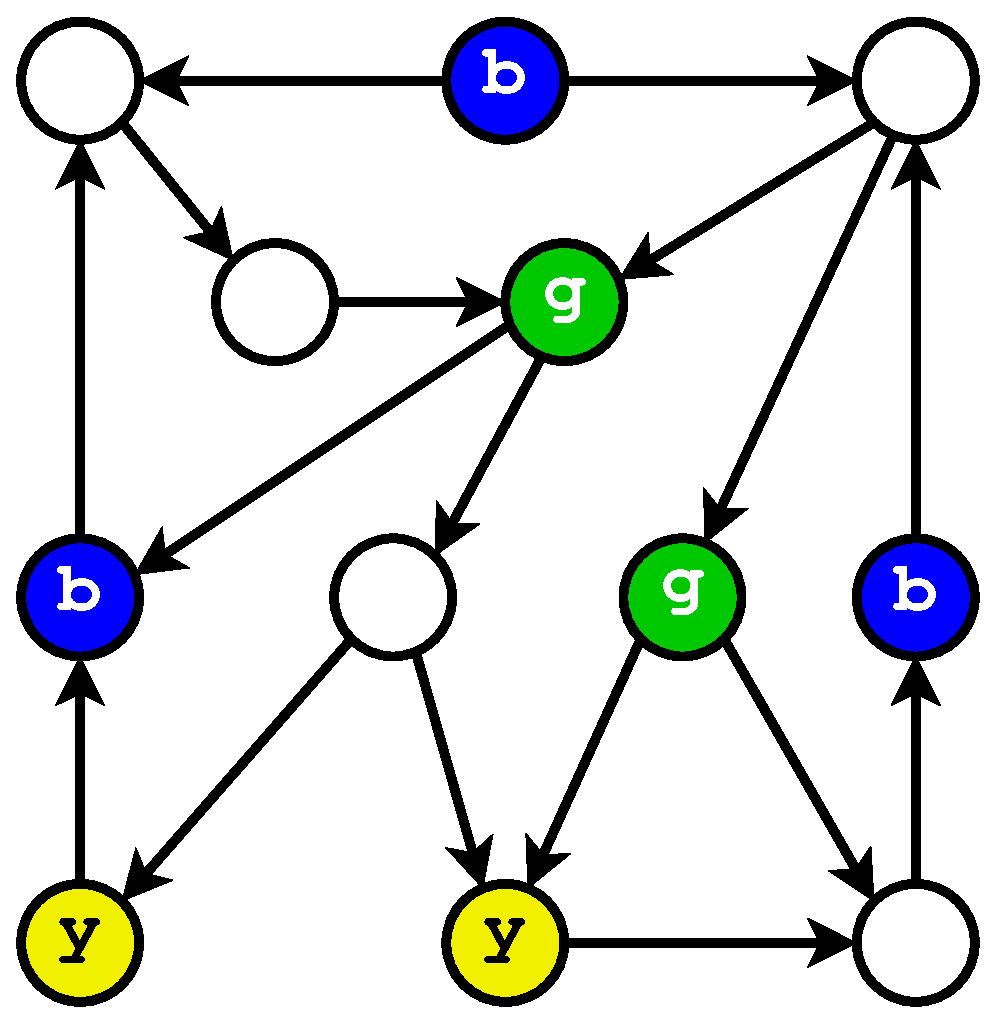
\includegraphics[width=0.75\linewidth]{images/nutshell-answer.eps}
  \caption{Example of an operationally colored graph.}
  \label{fig:imp-ppa}
\end{subfigure}
\hfill
\begin{subfigure}[b]{0.4\textwidth}
  \centering
  \includegraphics[width=0.4\textwidth]{images/nutshell-abstraction.eps}
  \vspace{3ex}
  \caption{Path predicate abstraction graph of Fig.~\ref{fig:imp-ppa}.}
  \label{fig:abs-ppa}
\end{subfigure}
\caption{Example of an Operational coloring of graphs. Implementation automata $M$ in~\ref{fig:imp-ppa} and its corresponding abstraction automata $\hat{M}$ in~\ref{fig:abs-ppa}. (Reprinted from \cite{paper-pdd})}
\label{fig:oper-graph}
\end{figure}

As stated in \cite{paper-pdd}, the coloring of the operational graph has the following attributes:

\begin{itemize}
\item All operational paths are finite. Hence, every cycle in the graph must include at least one colored node. 
\item All nodes of the same color allow for the same set of operation. In other words, if there exists an operational path from node colored $A$ to node colored $B$, then, for any node colored $A$, there is an operational path to some node colored $B$.
\end{itemize}

This “\textit{operational coloring}” allows the abstraction of the implementation graph. Since the colored nodes of the same color support the same operations, they can be abstracted as a single node. In addition, the white nodes are removed, and all corresponding operations collapsed into a single edge. As a result, an abstraction graph can be derived from the implementation graph and they both comprise the same set of operations, i.e. they are equivalent.

The direct graphs may be interpreted as a finite state transition structure such as Kripke Model or an FSM. In \cite{paper-pdd} the Kripe models are translated into FSMs. Then, the Kripke states become a set of three separated coloring functions applied to objects of the RTL implementation:

\begin{enumerate}
    \item A function that maps a subset of the FSM states to states colors $\hat{S}$;
    \item A function that maps input sequences to input colors $\hat{X}$ ; 
    \item A function that maps output sequences to output colors $\hat{Y}$.
\end{enumerate}

These colors serve as elements of an abstract FSM $\hat{M} = (\hat{S}, \hat{s}_{reset}, \hat{X}, \hat{Y}, \hat{\delta}, \hat{\lambda})$. Reading the graph in Fig.~\ref{fig:oper-graph} as an FSM, it means that, for any sequence of input colors, the implementation FSM and the abstract FSM produce the same sequence of output colors. This is called “\textit{sequential equivalence in terms of colors}”.

Even though the abstraction, i.e. the coloring, can be done in different ways, the coloring functions have to follow the operational coloring requirements stated in \cite{paper-ppa}.

Finally, as stated in \cite{paper-pdd}, in practice, the operational coloring is established through formal property checking. Thus, every operation of the design must be described as a property, creating a complete set of operation properties. Any property that can be expressed in terms of colors will be valid for both abstraction and implementation.

\subsubsection*{SystemC-PPA}

\textit{SystemC-PPA} is a subset of \textit{SystemC} \cite{lib-systemc}. According to Ludwig et al. \cite{paper-pdd}, the restriction to a subset is needed because \textit{SystemC} lacks clear semantics with respect to modelling digital hardware. Writing SystemC-PPA compliant modules results in an executable system-level design that also matches the semantic of the formal model of \cite{paper-pdd}. The usage of SystemC-PPA and how it is inserted on the PDD flow is detailed in Sec.~\ref{subsection:PDD-flow}.

The way a SystemC-PPA module is structured allows its behaviour to be extracted as a PPA. In order to achieve that, modules should adhere to the following guidelines:

\begin{enumerate}
    \item model an FSM in a time-abstraction fashion;
    \item have a single thread executing infinitely;
    \item communicate only through an allowed set of communication interfaces;
    \item only block upon a call to a blocking communication interface;
    \item not have cyclic execution path without blocking communication;
    \item use only objects whose size is known at compile time.
\end{enumerate}

As stated in the guidelines, SystemC-PPA modules are allowed to a specific set of communication interfaces, or \textit{ports}. There are three kinds of ports available that aim to provide enough flexibility to model any type of hardware communication at the RTL level. The first one is the \textit{blocking} interface which implements a blocking message passing \textit{handshake}, and it ensures that there is no message loss. The second type is called \textit{Master/Slave} interface. It should be used when the slave side is known to be always ready to communicate. In this case, the master side may communicate without having to synchronize. The last type is named \textit{Shared} interface which does not implement any \textit{handshake} mechanism. Therefore, the \textit{Shared} interface is able to model the behaviour of volatile memory and it fits for modelling unordered input data like sensor values. 

\begin{figure}[htb!]
    \begin{lstlisting}[language=C++]
    struct Example : public sc_module {
        //Constructor
        Example (sc_module_name name):
            value(9) {SC_THREAD (fsm);}
        SC_HAS_PROCESS(Example);
    
        //Ports
        blocking_in<int> b_in;
        blocking_out<bool> b_out;
    
        //Variables
        int value;
    
        //Finite State Machine
        void fsm(){
        while(true){
            b_in->read(value);
            if (value < 10){
                b_out->write(true);
            }else b_out->write(false);
        }}
    };\end{lstlisting}
    \caption{Example of a module written in SystemC compliant to the SystemC-PPA semantics. The module is intended as a toy example and simply reads a integer value through a \textit{blocking} port, and writes \textit{true} to a Boolean output, also of the \textit{blocking} type, if the value is lower than 10 or writes \textit{false} otherwise. }
    \label{fig:sysc-example}
\end{figure}

Fig.~\ref{fig:sysc-example} shows an example of a SystemC-PPA module extracted from \cite{descam}. The module has a single thread that runs infinitely, called\textit{ fsm()}. There are two communicating ports of the \textit{blocking} interface type; an input $b\_in$ and an output $b\_out$. These ports allow the module to communicate through blocking method-calls, for instance, the \textit{read()} and \textit{write()} at lines 17 and 19. 

To conclude, SystemC-PPA does not place any restrictions on which types of hardware behaviour can be modelled, but \textit{how} it should be described.

\subsection{The PDD flow}
\label{subsection:PDD-flow}

The complete flow of the Property-Driven Design methodology proposed in \cite{paper-pdd} is depicted in Fig.~\ref{fig:pdd-flow}. The starting point for the design process is an ESL description of the system. Already in the system-level, first refinements should be made in order to create a system-level model from which the PPA can be extracted, i.e. clear semantics with respect to PPA, or a SystemC-PPA compliant description. This refined description is said to be at the \textit{architectural-level}. 

\begin{figure}[htb!]
	\centering
	\includegraphics[width=0.85\textwidth]{images/design-flow.pdf}
	\caption{Design flow for the PDD methodology. (Reprinted from \cite{paper-pdd})}
	\label{fig:pdd-flow}
\end{figure}

At the architectural-level, the system behaviour is described in terms of data manipulation between communication points. In other words, the important states corresponds to the communication transactions, and an operation describes the data path between communication points. The communication is modelled in a time-abstract way. 

The second step of the design flow starts with the generation of abstract properties. Each property specifies an operation of the design, and for each module of the system, a set of properties is generated. These properties describe the \textit{I/O} behaviour that maps the communication primitives employed in the abstract design to the corresponding communication schemes at the RTL, as detailed in \cite{paper-pdd}. There are three types of properties generated for the property set in this step:

\begin{enumerate}
\item Reset Property: it is a special operation that describe the design behaviour and state after reset.
\item Regular Property: describe the behavior of a regular operation between communication points.
\item Wait Property: generated for each blocking port. Upon the wait for a synchronization signal in a blocking message transfer, this operation guarantees that the design remains at the same state.
\end{enumerate}

For the third step, the design flow splits into two threads. The thread on the left side of Fig.~\ref{fig:pdd-flow} refers do the RTL design process which defines the implementation of a \textit{cycle-accurate} RTL design from an abstract implementation. This corresponds to the conventional RTL design process, and all common design practices can be applied. In addition, any solution regarding the micro architectures of the system can be chosen.

The thread on the right side of Fig.~\ref{fig:pdd-flow} formally describes what is implemented by the left side through a set of properties that constitute a “\textit{formal data sheet}” of the design. This formal description provides the formal proofs that anchor the soundness of the system model and therefore the correctness of the design refinements. The properties are initially generated in terms of macros and functions. During this step of the design process, a \textit{refine-and-implement} cycle is established between the two threads. While the RTL is implemented, the property set must be refined to include the implementation details by updating the generated macros and functions. In order to ensure the correct refinement, the designer must change the properties by filling this set of fields.

During the \textit{refine-and-implement} process, the property suite can be checked against the RTL implementation, and found mismatches can be debugged. The system-level description is a sound path predicate abstraction of the RTL design, guaranteed by formal verification, when at least all the generated properties have been proved correct on the RTL code.

\subsubsection*{DeSCAM}

The authors in \cite{paper-pdd} have implemented a tool to support PDD methodology, called \textit{DeSCAM} (Design from SystemC Abstract Models) \cite{descam}. This tool is primarily essential on the step two of PDD flow for automatically generating the abstract property suit. However, it was designed in order to assist the designer through the entire PDD flow.

Starting with an abstract ESL description of the system, the tool can analyse and give the designer feedback to help refining the initial system-level model into a model at the architectural-level, which is PPA compliant. After having a correct SystemC-PPA description of the system, DeSCAM automatically generates the abstract property set to be refined by the designer. To assist even further, DeSCAM can optionally generate templates in HDL for the main control structures of the system that can be used as a starting point for the RTL implementation.

For each type of communication interface, the tool will generate a specific set of signals for both properties macros and HDL template. A \textit{blocking} interface will generate one signal of the port datatype for transporting the message content, and two more synchronization Boolean signals to implement the four-phase \textit{handshake} behaviour. One outgoing signal to start the handshake tagged with the \textit{notify} suffix, and a incoming signal tagged with the \textit{sync} suffix which informs that the other side is ready to communicate. The \textit{Master/Slave} interface only needs the data signal for the message and one synchronization signal; an outgoing \textit{notify} for the \textit{Master} port and incoming \textit{sync} for the \textit{Slave} port. The \textit{Shared} interface does not require any synchronization signal.

Regardless the of facilitation provided by the tool, the PDD methodology proposed in \cite{paper-pdd} can be applied without any restrictions on the RTL design with respect to architecture, implemented functionality, micro architectural optimizations and coding style. 

\newpage
% ----------------------------------------------------------
% Verification of Pipelined Processors
% ----------------------------------------------------------
\chapter{Verification of Pipelined Processors}
\label{chapter:pipeline}

This chapter presents a brief discussion on how IPC can be used to verify a pipelined processor. First, the concept of \textit{Pipelining} is reviewed with its main characteristics in Sec.~\ref{section:pipe-overview}. Then, an introduction on how to create an operational description of a pipelined processor along with a property example is presented in Sec.~\ref{section:ipc-pipe-processor}. Next, the notion of completeness for pipelined processors is discussed, including an introduction to the \SSQED{} approach, in Sec.~\ref{section:s2qed}. Finally, a discussion about the PDD method for Pipelined Processors is presented in Sec.~\ref{section:pdd-pipe-processor}.  

\section{Overview of Pipelined Processors}
\label{section:pipe-overview}

\textit{Pipelining} is a technique used to allow overlapping execution of instructions in a single core of a processor \cite{book-comp-org}. Instead of having instructions executing one after another in a sequential manner, the execution path for the instruction is divided into steps, called \textit{pipeline stages}. Thus, multiple instructions can overlap in time, each one executing in a different stage of the pipeline, Fig.~\ref{fig:pipe-example}.

\begin{figure}[htb!]
	\centering
	\includegraphics[width=0.85\textwidth]{images/pipeline-example.PNG}
	\caption{Illustration of the execution of instructions in a nonpipelined processor (top) versus pipelined execution (bottom). The \textit{ld} instruction loads data from the memory into a register in the processor register file. In this example, memory \textit{stalls} are not considered. (Reprinted from \cite{book-comp-org})}
	\label{fig:pipe-example}
\end{figure}

Since different types of instructions have very similar execution \textit{steps}, each step on the data path can be turned into a pipeline stage. For example, a common partition adopted in different pipelined processor implementations is: 

\begin{itemize}
\item Instruction Fetching (\textit{IF}): fetches a new instruction from memory to feed the pipeline;
\item Instruction Decoding (\textit{ID}): decodes instruction \textit{opcodes} and reads its operands from the register file;
\item Execution (\textit{EX}): executes the instruction operation. Usually associated with ALU operations;
\item Data Access (\textit{MEM}): performs \textit{read} and \textit{write} operations with data memory;
\item Write back (\textit{WB}): writes back the operations results or loaded data from data memory.
\end{itemize}

Certainly, each processor can have its own pipeline implementation, but they usually constitute some variation of the five presented stages.

One main advantage of pipelining is increasing the instruction \textit{throughput}, the amount of processed data per time unit. This advantage is illustrated in Fig.~\ref{fig:pipe-example}. In this example, a single \textit{load} instruction takes 800\,ps in a nonpipelined processor. Considering a pipelined processor with the five aforementioned stages, and with each stage taking 200\,ps, the three \textit{load} instructions execute in 1400\,ps, in contrast to the 2400\,ps needed for the nonpipelined processor. In this example, of course, possible \textit{stalls} caused by waiting for data memory are not considered for simplicity reasons. 
\TLSAY{If the frequency remains the same non-pipelined would be better because we get 1 instruction / cycle where as in pipelined we get (1/number of stages) instructions / cycle. 
Right? } \SSSAY{Not really. Once the pipeline is filled, you still get one instruction done per cycle. In any case, since it is a brief overview about pipeline. I thought of only using this really simple example to ilustrate and not going into so much details.}

\section{Property Checking for Pipelined Processors}
\label{section:ipc-pipe-processor}

In order to verify the design by property checking, the processor behaviour has to be described in term of operations, see Sec.~\ref{section:formal-verification}. There are many ways to achieve that, but one simple and intuitive way is to consider an operation as the complete execution of an instruction through all the pipeline stages. This operational description is more intuitive because the behaviour of each instruction is already specified in the \textit{Instruction Set Architecture}~(ISA) of the corresponding implemented processor, and it is simpler than specifically describing different combinations of instructions at different pipeline stages at time.

Since every operation starts and ends at an \textit{important state}, a common pipeline stage can be chosen as the initial and final state. As an example, one may consider the \textit{IF} stage as the important state and that every operation starts being fetched and ends when the next instruction is fetched. In practice, when the \textit{Instruction Under Verification}~(IUV) moves from \textit{IF} to \textit{ID}, the next instruction is already fetched.

A complete set of properties needs to prove all \textit{outputs} and \textit{visible registers} at all times, see Sec.~\ref{subsection:notion-completeness}, according to determination requirements. For this operational description of pipelined processor, one property will prove \textit{outputs} and visible registers corresponding to each pipeline stage. Consider the property in Fig.~\ref{fig:ex-add-ppt}. It depicts an example of a property proving the \textit{ADD} instruction in a 4-stages pipeline processor. The \textit{Program Counter} (PC) is proven only at the \textit{ID} stage, $t\_ID$. This does not compromise the completeness if there is always a property proving PC at all times. For example, at $t\_IF$ the previous instruction is at the \textit{ID} stage and proves the PC, and at $t\_EX$ is the instruction succeeding the IUV which is at the \textit{ID} stage proving the PC.

\begin{figure}[htb!]
    \begin{lstlisting}
    property ADD;
    assume:
        //conceptual state
        at t_IF: conceptual_state;
        at t_IF: empty_pipeline;
    
        //Trigger
        at t_IF: instr_type(fetched_instr) == ADD;
    prove:
        at t_ID: conceptual_state;
        at t_ID: PC == PC_at_t_IF + 4;
    
        at t_EX: ALU_oper_a == getOperA(fetched_instr);
        at t_EX: ALU_oper_b == getOperB(fetched_instr);
        at t_EX: ALU_result == ALU_oper_a + ALU_oper_b;
        
        at t_WB: regile_wb == ALU_result;
    
        at t_end: REGFILE(reg_dest) == ALU_result;
    end property;\end{lstlisting}
    \caption{Example of a property describing the execution of the \textit{ADD} instruction in a pipelined processor.}
    \label{fig:ex-add-ppt}
\end{figure}

In the example property for an \textit{ADD} instruction in Fig.~\ref{fig:ex-add-ppt}, the processor \aTLSAY{The processor is now a computational model. We select all states that relate to the conceptual state} \aSSSAY{Sorry, I did not understand this comment :(} is in a state called \textit{conceptual\_state} at $t\_IF$ \SSREP{, line 4}{(see line 4)} \aTLSAY{dont do this , line~x ... rather do ... Line 4, shows ... In line 4 xyz ... or (see line~x)}. This conceptual state corresponds to a state where the processor is ready to fetch a new instruction. When the IUV is at the \textit{ID} stage, the processor should be again at the conceptual state and ready to fetch a new instruction, as shown in line 10. Back to the assumptions, the property states that the fetched instruction is of type \textit{ADD}. In the commitments, the visible register PC is proved to be incremented by four at $t\_ID$. At $t\_EX$, the property proves that the ALU receives the right operands and computes the right result. At $t\_WB$, the right result is sent back to the register file. Finally, at $t\_end$, the destination register in the register file holds the right computed result.

A property set that covers the \textit{reset} behaviour and has one property for every possible instruction in the ISA will pass the completeness tests for successor, determination, and reset (see Sec.~\ref{subsection:notion-completeness}). However, the case-split test will not hold. This is because the properties referred so far assume that the IUV execution is not influenced by any other instruction in the pipeline. Line 5 in the listing of Fig.~\ref{fig:ex-add-ppt} assumes that the pipeline is empty when the IUV is fetched. Obviously, in practice this will hardly be the case. In order to overcome this problem, an approach called \SSQED{} \cite{paper-symbolic} can be employed. The next section presents an overview of this approach.

\section{Completeness with \SSQED{}}
\label{section:s2qed}

\SSQED{} \cite{paper-symbolic} is a verification approach based on a bounded model with symbolic initial state. It offers a proof that the execution of each instruction is independent of its \textit{program context}. In other words, each instruction executes independently of other instructions currently in the pipeline. 

Errors in hardware design are often called “\textit{bugs}” or “\textit{logic bugs}”. In \cite{paper-gapfree}, these errors are defined as a deviation of the implementation’s behaviour from the specification. Also in \cite{paper-gapfree}, two categories of logic bugs are presented:

\begin{enumerate}
\item Single-instruction bug: it is defined when the \textit{opcode} and the operands of the IUV causes an error in all program contexts, i.e. independently of all previously executed instructions.
\item Multiple-instruction bug: it is defined when it is not a single-instruction bug and there exists an instruction \textit{opcode}, a set of operands and a program context such that the execution of the IUV leads to an error.
\end{enumerate}

The property set presented so far, composed with properties like the one in Fig.~\ref{fig:ex-add-ppt}, is able to identify single-instruction bugs since they are independent of the program context. Therefore, the \textit{empty\_pipeline} assumption will not interfere on finding these types of errors. On the other hand, this assumption will mask multiple-instruction bugs as they require specific instruction sequence scenarios in order to occur.

In order to exemplify a multiple-instruction bug, consider a \textit{read-after-write} hazard. This hazard happens, for example, when an instruction \textit{reads} a register that is written by its immediate previous instruction. In this case, considering the same 4-stages pipeline, the register value is read before the "write to the register file" operation is complete by the previous instruction. To avoid an error, pipelined processors implement a mechanism called \textit{forwarding}. This mechanism forwards the value that is going to be written in the register file to previous pipeline stages, so it can be used by the following instruction if needed. A bug in the forwarding structure is considered a multiple-instruction bug as it does not depend only on the IUV, but in previous instruction fed into the pipeline. 

The \SSQED{} approach covers multiple-instruction bugs by assigning one same instruction, at an arbitrary time point, to execute in two \textit{identical} and \textit{independent} instances of the processor under verification. The computational model of the \SSQED{} approach is depicted in Fig.~\ref{fig:s2qed-model}.

\begin{figure}[htb!]
	\centering
	\includegraphics[width=0.7\textwidth]{images/s2qed_model.pdf}
	\caption{\SSQED{} computational model. Both constrained and unconstrained instances, \textit{CPU1} and \textit{CPU2} respectively, execute the same IUV. (Reprinted from \cite{paper-gapfree})}
	\label{fig:s2qed-model}
\end{figure}

The first CPU instance, in the same manner as the CPU model considered so far, is constrained to execute the IUV in an empty pipeline. The second CPU instance is unconstrained to execute an arbitrary sequence of instructions. The only restrictions for the second CPU instance are that it fetches the same instruction as the first instance at time $t$, and they both are consistent. This required consistency, named \textit{QED-consistency}, is defined in \cite{paper-gapfree} as follows:

\begin{quote}
     \textit{"In the \SSQED{} computational model, the two CPU instances are QED-consistent at a time $t$, if the corresponding architectural state elements of both instances at time point $t$ hold the same values."}
\end{quote}

For this \SSQED{} computational model, the SAT-Solving tool will compare the execution of the IUV in the constrained empty pipeline of the first CPU instance with all the scenarios for the unconstrained execution of the IUV in the second CPU instance, including the context where the multiple-instruction bugs appear and propagate. The listing on Fig.~\ref{fig:ex-s2qed-add-ppt} shows an example of an \SSQED{} property for an \textit{ADD} instruction.

\begin{figure}[htb!]
    \begin{lstlisting}
    property S2QED_ADD;
    assume:
        // constraints on CPU1
        at t_IF: cpu1_conceptual_state;
        at t_IF: cpu1_empty_pipeline;
        during [t_IF+1, t_WB]: instr_type(cpu1_fetched_instr) == NOP;
    
        // same IUV
        at t_IF: cpu1_fetched_instr == cpu2_fetched_instr;
        at t_IF: instr_type(cpu1_fetched_instr) == ADD;
    
        // QED consistent registers
        at t_WB: qed_consistency_registers();
    
    prove:
        at t_end: qed_consistency_registers();
        end property;\end{lstlisting}
    \caption{Example of a \SSQED{} property describing an \textit{ADD} instruction as the IUV.}
    \label{fig:ex-s2qed-add-ppt}
\end{figure}

Lines 4 and 5 of the property in Fig.~\ref{fig:ex-s2qed-add-ppt} constrain the \textit{CPU1} instance to be on the conceptual state and have an empty pipeline. The assumption in line 6 constrains the \textit{CPU1} to fetch only \textit{NOP} instructions after fetching the IUV. This assumption is not crucial to prove the model, however, it reduces unnecessary complexity for the SAT-solving tool. The assumptions on lines 9 and 10 will bind the IUV in both CPU instances to be the same and of type \textit{ADD}. Finally, the last assumption on line 13 comprises the QED-consistency, which is also proven on the commitment on line 16.

The macro function \textit{qed\_consistency\_registers()} expresses the Boolean function shown in Eq.~\ref{eq:consistency-register}. It characterizes the QED-consistency register state for a processor with $N$ registers on its register file.

\begin{equation}
    qed\_consistency\_registers := \,\, \bigwedge_{i = 0}^{N-1} \left(R^i_{cpu1} = R^i_{cpu2}\right)
    \label{eq:consistency-register}
\end{equation}

The consistency between the two CPU instances is the key for accomplishing completeness solving the case-split test. The \SSQED{} computational model guarantees a consistent result of every operation between both instances. Therefore, proving the case-split test for one of the instances is sufficient.

The case-split test is easy to satisfy for a set of \SSQED{} properties, since every possible instruction sequence is implicitly considered on the \textit{CPU2} instance. For a formalism on how the case-split test is proven on a \SSQED{} property set, the reader may refer to \cite{paper-gapfree}.

\section{PDD for Pipelined Processors}
\label{section:pdd-pipe-processor}

The Property-Driven Design approach, see Sec.~\ref{section:PDD}, generates operational properties from an ESL design described in SystemC-PPA in order to prove that the later implemented RTL design is sound with respect to the ESL. The SystemC-PPA description is a sequential model from which the extracted operations represent transitions between important states. 

A pipelined processor will have its operations overlapping in time, for each operation represents an instruction executing throughout the pipeline stages. Consequently, while the ESL model describes the behaviour of instructions of a program executing sequentially one after another in the processor (see the execution on top of Fig.~\ref{fig:pipe-example}) the RTL implements the pipeline where an instruction starts executing before the previous one is completed. This concurrent behaviour is shown on the bottom of Fig.~\ref{fig:pipe-example}.

If the ESL model does not describe the concurrent execution of operations, the generated PPA will not match the pipeline implemented in the RTL. In practice, the DeSCAM tool (see Sec.~\ref{subsection:PDD-flow}), that generates the properties, derives the important states from communication transactions in the DUV, so the operations represent the data manipulation between communication. 

Let us consider the 4-stage pipeline processor defined in this chapter with two communicating interfaces. One memory interface to fetch instructions and the other for communication with the data memory. Fig.~\ref{fig:ppa-seq} shows the PPA extracted from the sequential SystemC-PPA description of the processor. 

\begin{figure}[htb!]
	\centering
	\includegraphics[width=0.6\textwidth]{images/PPA_old.pdf}
	\caption{PPA for a sequential SystemC-PPA processor description.}
	\label{fig:ppa-seq}
\end{figure}

The bigger circles in the PPA of Fig.~\ref{fig:ppa-seq} represent important states where there is some transaction with a communication port, while the smaller circles represents unimportant states. There are two important states, the \textit{IF} state that communicates with the instruction memory, and the \textit{MEM} state that communicates with the data memory.

The listing of Fig.~\ref{fig:ex-pdd-add-ppt} shows an example of a property generated for an \textit{ADD} instruction from a sequential ESL. The time $t$ corresponds to the fetching time, and the time $t\_end$ to the time point after the write back, $t+4$. The property is triggered when the CPU is ready to fetch, \textit{conceptual\_state}, and a new instruction of type \textit{ADD} is fetched. At $t\_end$, after the \textit{ADD} instruction is completely executed, the commitments prove that the right result is written to the right destination register.

\begin{figure}[htb!]
    \begin{lstlisting}
    property PDD_ADD;
    assume:
        at t: conceptual_state;
        at t: instr_type(fetched_instr) == ADD;
    prove:
        at t_end: conceptual_state;
        at t_end: PC == PC_at_t + 4;
        at t_end: REGFILE(reg_dest) == ADD_result;
        
        //intruction memory interface
        during [t+1, t_end-1]: instr_req_out_notify == false;
        at t_end: instr_req_out_notify == true;
        
        //data memory inteeface
        during [t+1, t_end]: data_req_out_notify == false;
    end property;\end{lstlisting}
    \caption{Example of a property for the \textit{ADD} instruction generated from a sequential PPA.}
    \label{fig:ex-pdd-add-ppt}
\end{figure}

It is important to notice that the request signal to fetch a new instruction is only asserted at the time point $t\_end$, being set to false during the whole instruction execution time. Similarly, the request signal for the data memory is de-asserted all the time since the \textit{ADD} instruction does not communicate with the data memory at any time. As a result, a set with $n$ properties corresponding to the $n$ instructions of the processor ISA will not hold for the RTL design. One problem can be easily spotted in this example. Consider the operation property for a \textit{LOAD} instruction, while the \textit{ADD} property tries to prove that the \textit{data\_req\_out} signal is always false, the \textit{LOAD} instruction tries to prove that the same signal is set to true during the memory phase.

Two approaches could be considered in order to apply the PDD flow for the design of a pipelined processor. First, the designer can redesign the ELS description so that it reflects the pipeline concurrent RTL behaviour. In this case, the ESL abstraction is lost because RTL implementation details are replicated at the ESL model. The second alternative is refining the pipeline within the macros for the generated instructions. Once again, the designer would have to replicate part of the RTL implementation, this time during the refinement of the macros. 

For both approaches, additional effort by the designer is required, which mitigates the goal of applying the PDD method, that is to accelerate the design process. Chapter~\ref{chapter:algorithm} presents how the PDD approach can be extended for pipelined processors by introducing small changes at the SystemC-PPA, and proposes an algorithm that can be used to convert the generated DeSCAM properties into a property set that matches the pipeline concurrent behaviour. 


\newpage
% ----------------------------------------------------------
% The Pipeline Algorithm
% ----------------------------------------------------------
\chapter{The Pipeline Algorithm}
\label{chapter:algorithm}

The current chapter presents how the PDD flow can be extended in order to support the design of pipelined processors in Sec.~\ref{section:extend-pdd}. Sec.~\ref{section:pipe-algorithm} introduces the Pipeline Algorithm to generate a set of Pipeline Properties. Finally, in Sec.~\ref{section:plugio-s2qed-top}, a plugin for \textit{DeSCAM} to assist on the \SSQED{} environment setup is presented. 

\section{Extending the PDD flow for Pipelined Processors}
\label{section:extend-pdd}

The Property-Driven Design flow presented on Sec.~\ref{subsection:PDD-flow} can be extended to help the hardware designer to deal with pipelined processors. The original PDD flow is depicted on the left side of Fig.~\ref{fig:new-pdd-flow}. On the right side, an extended PDD flow is presented with two additional steps that are included to support pipelined processors: insert stages and pipeline algorithm. 

\begin{figure}[htb!]
	\centering
	\includegraphics[width=0.85\textwidth]{images/new_pdd_flow.pdf}
	\caption{On the left, property generation with \textit{DeSCAM} for the original PDD flow. On the right, extension of the PDD flow to better support of pipelined processors.}
	\label{fig:new-pdd-flow}
\end{figure}

In the same manner as the original flow, the extended PDD flow starts with a description at the architectural-level, which is PPA compliant. Before applying the description to \textit{DeSCAM}, the SystemC-PPA model is modified to include information about the pipeline behaviour resulting in an enhanced PPA description. This description can be applied to \textit{DeSCAM} which will generate a sequential property set of \textit{micro properties} (to be detailed later in this section). Finally, the \textit{Pipeline Algorithm} can merge the \textit{micro properties} generating a property set with \textit{pipeline properties}.

The \textit{Insert Stages} phase allows the designer to include information about the desired pipeline structure into the SystemC-PPA model. It is important to emphasise that the designer does not have to translate the concurrent pipeline behaviour from the RTL implementation into the ESL model. The designer needs simply to include information about the desired pipeline stages at the appropriate points. This is done by calling the function \textit{insert\_state()} at the points in the data path of the ESL model corresponding to each pipeline stage. This function call will not influence on the sequential behaviour of the simulation for the model at the system-level.

The \textit{insert\_state()} function is interpreted by the \textit{DeSCAM} tool as a directive to include an important state in the PPA for that respective position in the code. Without this directive, the important states were only generated for communication calls, which affects the \textit{I/O} behaviour (see Sec.~\ref{subsection:PDD-flow}). Consider the regular PPA in Fig.~\ref{subfig:ppa-seq} extracted from a sequential ESL model without the manually inserted stages. If a call to insert a state for each pipeline stage is used, the resulting enriched PPA such the one in Fig.~\ref{subfig:ppa-pipe-processor} is obtained.

\begin{figure}[htb!]
\centering
\begin{subfigure}[b]{0.45\textwidth}
  \centering
	\includegraphics[width=0.9\textwidth]{images/PPA_old.pdf}
	\caption{PPA for regular PDD flow.}
	\label{subfig:ppa-seq}
\end{subfigure}
\hfill
\begin{subfigure}[b]{0.45\textwidth}
  \centering
	\includegraphics[width=0.9\textwidth]{images/PPA_new.pdf}
	\caption{PPA for extended PDD flow.}
	\label{subfig:ppa-pipe-processor}
\end{subfigure}
\caption{(a) PPA for a sequential SystemC-PPA processor description like in Fig.~\ref{fig:ppa-seq}. (b) Enriched PPA for an enhanced SystemC-PPA processor description with states inserted for each pipeline stage.}
\label{fig:ppa-old-and-new}
\end{figure}

The enriched PPA of Fig.~\ref{subfig:ppa-pipe-processor} derived from an enhanced SystemC-PPA has one important state for each pipeline stage. As a result, the property set generated by \textit{DeSCAM} will also be different. Let us consider an \textit{ADD} instruction for a 4-stage pipeline processor as an example. The property generated by \textit{DeSCAM} for a regular sequential SystemC-PPA description is seen in the listing of Fig.~\ref{fig:ex-pdd-add-ppt}. Since only one important state, for instance \textit{IF}, is present on the execution path of an \textit{ADD} instruction, only one property is generated for describing the behaviour of this instruction. This can be also seen on the PPA of Fig.~\ref{subfig:ppa-seq} where the \textit{ADD} operation corresponds to a single edge starting  and ending on important state \textit{IF}. On the other hand, an \textit{ADD} instruction execution on the enriched PPA of Fig.~\ref{subfig:ppa-pipe-processor} corresponds to four edges. Therefore, four properties will be generated for this single instruction. These operations describing the behaviour between two pipeline stages are named \textit{micro operations}, or \textit{micro properties}. The listing on Fig.~\ref{fig:add-if-id-micro-ppt} shows two examples of micro properties. The property in Fig.~\ref{subfig:add-if-micro-ppt} corresponds to the operation between the \textit{IF} and \textit{ID} stages, and the property in Fig.~\ref{subfig:add-id-micro-ppt} the operation when the IUV goes from stage \textit{ID} to \textit{EX}.

\begin{figure}[htb!]
     \centering
     \begin{subfigure}[b]{\textwidth}
         \begin{lstlisting}
    property PDD_ADD_IF;
    dependencies: no_reset;
    for timepoints:
        t_end = t+1;
    freeze:
        PC_at_t = PC@t;
    assume:
        at t: IF;
    prove:
        at t_end: ID;
        at t_end: PC == PC_at_t + 4;
        at t_end: fetched_instr == instr_in_sig;
        at t_end: operands == getOperandsFromRegFile(fetched_instr);
        during [t+1, t_end-1]: instr_req_out_notify == false;
        at t_end: instr_req_out_notify == true;
        during [t+1, t_end]: data_req_out_notify == false;
    end property;\end{lstlisting}
         \caption{Micro property describing operation from \textit{IF} stage to \textit{ID} stage.}
         \label{subfig:add-if-micro-ppt}
     \end{subfigure}
     \hfill
     \begin{subfigure}[b]{\textwidth}
         \begin{lstlisting}
    property PDD_ADD_ID;
    dependencies: no_reset;
    for timepoints:
        t_end = t+1;
    freeze:
        PC_at_t = PC@t,
        fetched_instr_at_t = fetched_instr@t;
    assume:
        at t: ID;
        at t: getInstrType(fetched_instr) == ADD;
    prove:
        at t_end: EX;
        at t_end: PC == PC_at_t;
        at t_end: fetched_instr == fetched_instr_at_t;
        at t_end: ex_regData == operands.rs1 + operands.rs2;
        at t_end: ex_regAddr == operands.rd;
        at t_end: ex_regWrEn == true;
        during [t+1, t_end]: instr_req_out_notify == false;
        during [t+1, t_end]: data_req_out_notify == false;
    end property;\end{lstlisting}
         \caption{Micro property describing operation from \textit{ID} stage to \textit{EX} stage.}
         \label{subfig:add-id-micro-ppt}
     \end{subfigure}
        \caption{Example of micro properties generated for an \textit{ADD} instruction from an enhanced SystemC-PPA processor description with states inserted to each pipeline stage. The property in (a) refers to the transition between \textit{IF} and \textit{ID} stages, and the property in (b) the transition between \textit{ID} and \textit{EX}.}
        \label{fig:add-if-id-micro-ppt}
\end{figure}

One problem with describing the behaviour of a single instruction with multiple micro properties is the loss of intuitiveness for the designer. It is more natural to describe an instruction behaviour spawning over all pipeline stages. A second problem is that each micro operation generated will describe the behaviour of all \textit{outputs} and visible registers. As discussed in Sec.~\ref{section:pdd-pipe-processor}, this makes the property set impossible to hold because each property, in this pipelined processor context, should prove only the values of interest for the corresponding stage. An example of this problem can be observed in the micro properties of Fig,~\ref{fig:add-if-id-micro-ppt}. The PC behaviour is correctly proven to be incremented in (a) when the IUV is on the \textit{ID} stage. However, in (b), the PC is proven to remain with the same value. This is not true as the PC is normally incremented in every clock cycle as a new instruction is fetched. Another inconsistency refers to the output signal requesting a new instruction, \textit{instr\_req\_out\_notify}. In the  commitments of (b), the signal is proven to be de-asserted, which is not the expected behaviour of a pipeline processor that requests a new instruction every clock cycle when there is no \textit{stall}.

The other additional phase included on the extended PDD flow of Fig.~\ref{fig:new-pdd-flow} is the \textit{Pipeline Algorithm}. This proposed algorithm combines the micro properties referring to a single instruction into a \textit{pipeline property}. This property describes the behaviour of the instruction executing throughout all pipeline stages, similarly to the property shown in the listing of Fig.~\ref{fig:ex-add-ppt}. The Pipeline Algorithm is detailed in Sec.~\ref{section:pipe-algorithm}.

The notion of completeness discussed in Sec.~\ref{section:ipc-pipe-processor} and Sec.~\ref{section:s2qed} still applies. The set of pipeline properties generated by the algorithm represents the set of constrained properties that considers the IUV executing in a empty pipeline. For passing the case-split test and achieving completeness, a set of \SSQED{} properties has to be proven.

Finally, in addition to the HDL template that can be generated by \textit{DeSCAM} in order to assist the designer on the RTL implementation, see Sec.~\ref{subsection:PDD-flow}, a new plugin  for \textit{DeSCAM} was developed in this work. This plugin can be optionally used by the designer to automatically generate a top design in HDL creating the environment to prove the \SSQED{} properties. The plugin is detailed in Sec.~\ref{section:plugio-s2qed-top}.

\section{Generating the Pipeline Properties}
\label{section:pipe-algorithm}

The Pipeline Algorithm proposed in this work converts a property set of micro operations into a set of pipeline properties. Given a processor description at the architectural-level including the information of each pipeline stage by state insertion, the \textit{DeSCAM} tool will generate a sequence of properties for each instruction from the ISA of the processor model. The algorithm will merge the sequence of properties for each instruction into a single pipeline property. 

The listing in Fig.~\ref{fig:sysc-pipe-proc} shows an example of a SystemC-PPA compliant processor description. For simplicity, the presented ESL implementation omits some code such as variable declarations and function implementations. The purpose of this example is to illustrate one possible implementation of a 4-stages pipeline processor at the architectural-level that will be used throughout this section to help understanding the proposed algorithm.

\begin{figure}[htb!]
    \begin{lstlisting}[language=c++]
    class pipelined_processor : public sc_module {
        //ports for communication with instr mem
        master_in<unsigned int> instr_in;
        master_out<bool> instr_req_out;
        //ports for communication with data mem
        master_in<unsigned int> data_in;
        blocking_out<CUtoME_IF> data_req_out;
        void fsm() {
            nextsection = Sections::FETCH_PH;
            while (true){
                section = nextsection;
                if (section == Sections::FETCH_PH){
                    insert_state("IF");
                    instr_in->master_read(fetched_instr);
                    nextsection = Sections::DECODE_PH;
                } else if (section == Sections::DECODE_PH){
                    PC = PC + 4;
                    instr_req_out->master_write(PC);
                    operands = getOperFromRegFile(fetched_instr);
                    insert_state("ID");
                    nextsection = Sections::EXE_MEM_PH;
                } else if (section == Sections::EXE_MEM_PH) {
                    if (getInstrType(fetched_instr) == ADD) {
                        ex_regData = operands.rs1 + operands.rs2;
                        ex_regAddr = operands.rd;
                        ex_regWrEn = true;
                        insert_state("EX");
                    } else if (getInstrType(fetched_instr) == LOAD) {
                        ex_regAddr = operands.rd;
                        ex_regWrEn = true;
                        memAccess.addrIn = operands.rs1 + operands.imm; 
                        memAccess.wrEn = false;
                        data_req_out->write(memAccess, "MEM");
                        data_in->master_read(ex_regData);
                    } else {} //Other Instructions[...] 
                    nextsection = Sections::WRITEBACK_PH;
                } else if (section == Sections::WRITEBACK_PH) {
                    wb_regWrEn = ex_regWrEn;
                    wb_regAddr = ex_regAddr;
                    wb_regData = ex_regData;
                    insert_state("WB");
                    RegFile[wb_regAddr] = (wb_regWrEn) ? wb_regData : RegFile[wb_regAddr];
    }}}};\end{lstlisting}
    \caption{SystemC-PPA description of a 4-stage pipeline processor}
    \label{fig:sysc-pipe-proc}
\end{figure}

The \textit{pipelined\_processor} has two communication interfaces. One used to communicate with the instruction memory, and the other for data memory transactions. The instruction memory interface is of the type \textit{Master}, see Sec.~\ref{subsection:PPA}, and it has two signals. One \textit{output} for requesting a new instruction to a specific address, and an \textit{input} to read the instruction. The data memory interface also has two \textit{ports}. One \textit{blocking output} to send data request, and a \textit{Master input} to read the requested data from the memory.

The module has one main function called \textit{fsm()}, which runs infinitely and implements the behaviour of the processor. The variable \textit{section} keeps track of on which pipeline stage the current instruction is running. Starting from the \textit{FETCH\_PH} section, each instruction will execute in one pipeline stage at time. For each stage, the function \textit{insert\_state()} (lines 13, 20, 27 and 41) is called in order to create an \textit{important state} at the PPA extracted from this ESL model. Nonetheless, the simulation at the system-level is still sequential, and each instruction is only going to be executed after the previous one is finished.

The ESL model in the example depicts the behaviour of two instructions in specific: \textit{ADD} and \textit{LOAD}. The only implementation difference between them is at the \textit{EXE\_MEM\_PH} section, from line 23 to line 36. This section represents the \textit{EX} stage for the \textit{ADD} instruction, where a new state is inserted (line 27), and the computation of the addition operation with the respective operands is done (line 24). Observe that for the \textit{LOAD} instruction the manual insertion of a new instruction is not required because the data memory \textit{port} is of type \textit{blocking}. Therefore, this transaction demands a synchronization which is translated into a new important state when the PPA is generated. All the other sections are the same for both instructions. In the \textit{FETCH\_PH} phase, a new instruction if fetched from memory. In the \textit{DECODE\_PH} phase, the PC is incremented, and the \textit{opcode} and \textit{operands} are extracted from the fetched instruction. In the \textit{WRITE\_BACK\_PH} phase, the result from the ALU or the data fetched from the memory is written to the register file, line 42.

When this ESL model is parsed by \textit{DeSCAM}, a set of properties that comprises the \textit{reset property}, the regular properties and the \textit{wait properties} is generated. For the \textit{ADD} instruction, four micro properties are generated corresponding to the transitions between the pipeline stages \textit{IF}, \textit{ID}, \textit{EX}, \textit{WB} and back to \textit{IF}, i.e. each operation corresponds to an edge in the PPA of Fig.~\ref{subfig:ppa-pipe-processor}. Two of these micro properties are already shown in Fig.~\ref{fig:add-if-id-micro-ppt}. The property in (a) for the transition from \textit{IF} to \textit{ID}, and the property in (b) for the transition between \textit{ID} and \textit{EX}. The other two micro properties generated for the \textit{ADD} instruction are presented in Fig.~\ref{fig:add-ex-wb-micro-ppt}. These micro properties correspond to the transition (a) from \textit{EX} to \textit{WB}  and (b) from \textit{WB} to \textit{IF}. 

\begin{figure}[htb!]
     \centering
     \begin{subfigure}[b]{\textwidth}
         \begin{lstlisting}
    property PDD_ADD_EX;
    dependencies: no_reset;
    for timepoints:
        t_end = t+1;
    freeze:
        PC_at_t = PC@t,
        fetched_instr_at_t = fetched_instr@t;
    assume:
        at t: EX;
    prove:
        at t_end: WB;
        at t_end: PC == PC_at_t;
        at t_end: fetched_instr == fetched_instr_at_t;
        at t_end: wb_regWrEn = ex_regWrEn;
        at t_end: wb_regAddr = ex_regAddr;
        at t_end: wb_regData = ex_regData;
        during [t+1, t_end]: instr_req_out_notify == false;
        during [t+1, t_end]: data_req_out_notify == false;
    end property;\end{lstlisting}
         \caption{Micro property describing operation from \textit{EX} stage to \textit{WB} stage.}
         \label{subfig:add-ex-micro-ppt}
     \end{subfigure}
     \hfill
     \begin{subfigure}[b]{\textwidth}
         \begin{lstlisting}
    property PDD_ADD_WB;
    dependencies: no_reset;
    for timepoints:
        t_end = t+1;
    freeze:
        PC_at_t = PC@t,
        fetched_instr_at_t = fetched_instr@t;
    assume:
        at t: WB;
    prove:
        at t_end: IF;
        at t_end: PC == PC_at_t;
        at t_end: fetched_instr == fetched_instr_at_t;
        at t_end: RegFile[wb_regAddr] == (wb_regWrEn) ? wb_regData : RegFile[wb_regAddr];
        during [t+1, t_end]: instr_req_out_notify == false;
        during [t+1, t_end]: data_req_out_notify == false;
    end property;\end{lstlisting}
         \caption{Micro property describing operation from \textit{WB} stage to \textit{IF} stage.}
         \label{subfig:add-wb-micro-ppt}
     \end{subfigure}
        \caption{Example of micro properties generated for an \textit{ADD} instruction from an enhanced SystemC-PPA processor description with states inserted to each pipeline stage. The property in (a) refers to the transition between \textit{EX} and \textit{WB} stages, and the property in (b) the transition between \textit{WB} and \textit{IF}.}
        \label{fig:add-ex-wb-micro-ppt}
\end{figure}

The Pipeline Algorithm will convert the micro properties set into a pipeline properties set that comprises the \textit{reset} property, and merge the regular micro properties and \textit{wait} properties into pipeline properties. The refinement of the \textit{reset} property follows the regular property refinement of the PDD flow in \cite{paper-pdd}. Constraints can be added if needed, and the $t\_end$ must be updated to the appropriate time point.

The algorithm to merge the regular micro properties and \textit{wait} properties into a set of pipeline properties consists of three major steps:

\begin{enumerate}
\item \textit{Find the root state}: the \textit{root} state is the first important state to be reached by the system after \textit{reset}. This node within the PPA is used in step two as the start point for finding cycles;
\item \textit{Find cyclic paths}: In this step, all the cyclic sub-graphs of the PPA that start and end in the \textit{root} state are identified. For the PPA in Fig.~\ref{subfig:ppa-pipe-processor}, two cyclic paths are present, \textit{IF-ID-EX-WB-IF} and \textit{IF-ID-MEM-WB-IF}. The edges referring to the \textit{wait} operations are ignored in this step and converted into \textit{bounded wait for input} in step three.
\item \textit{Merging micro properties}: In this last step, the micro properties belonging to a cyclic path are converted into a single pipeline property. The algorithm to merge micro properties within the same cycle is detailed next. 
\end{enumerate}

\subsection*{The Merging Algorithm}

The procedure for merging a sequence of micro properties referring to the operations in a cyclic sub-graph of the PPA is presented in the flowchart in Fig.~\ref{fig:algorithm-flow}. The syntax employed for the algorithm corresponds to the proprietary language ITL \cite{onespin} because this syntax is more intuitive and readable than SVA for example. Nonetheless, the procedure can be easily adapted to other verification languages. 

\begin{figure}[htb!]
	\centering
	\includegraphics[width=0.7\textwidth]{images/algorithm.pdf}
	\caption{Flowchart for the merging algorithm that combines a sequence of micro properties of a cyclic sub-graph of the PPA into a Pipeline Property.}
	\label{fig:algorithm-flow}
\end{figure}

The first step of the merging algorithm is \textbf{Add Constraints}. As shown in the micro properties of Fig.~\ref{fig:add-ex-wb-micro-ppt}, \textit{DeSCAM} generates the properties already including one constraint, \textit{no\_reset}. This constraint informs the \textit{property checking tool} that, for the duration of the operation, there should be no \textit{reset} signal. At this step, the designer must include any other constraints that are valid for the entire duration of the operation. One example is a constraint that specify the memory protocol, so the tool knows how the memory \textit{input} signals behave.

For the \textbf{Add Timepoints} step, one timepoint variable is created referring to the commitments of each micro property. The micro properties include the $t\_end$ timepoint variable, see line 4 of Fig.~\ref{subfig:add-if-micro-ppt}, and these timepoints are integrated to the resulting pipeline property, e.g. $t\_id$, $t\_ex$, and $t\_wb$ representing the time for each pipeline stage.

Next, the cyclic path is analysed in order to identify if there are \textit{wait} operations present. If that is the case, the step \textbf{Add bounded wait to corresponding timepoint} is executed, where each \textit{wait} operation must be converted into a \textit{bounded wait} to the corresponding \textit{input} signal and included for the right timepoint. The micro properties in Fig.~\ref{fig:load-mem-wait-micro-ppt} show the transitions for a \textit{LOAD} instruction at the \textit{MEM} stage. In (a) the IUV is at stage \textit{MEM} and the \textit{sync} signal from the memory arrives. Then, the \textit{LOAD} instruction moves forward to the \textit{WB} stage. In (b), the wait operation proves that the IUV remains at the \textit{MEM} stage until the \textit{sync} signal comes. In this case, a \textit{bounded wait} for the \textit{input} signal \textit{data\_req\_out\_sync} is created at $t\_wb$, i.e. the timepoint corresponding to the write back stage.

\begin{figure}[htb!]
     \centering
     \begin{subfigure}[b]{\textwidth}
         \begin{lstlisting}
    property PDD_LOAD_MEM;
    dependencies: no_reset;
    for timepoints:
        t_end = t+1;
    freeze:
        PC_at_t = PC@t,
        fetched_instr_at_t = fetched_instr@t,
        data_in_sig_at_t = data_in_sig@t;
    assume:
        at t: MEM;
        at t: data_req_out_sync;
    prove:
        at t_end: WB;
        at t_end: PC == PC_at_t;
        at t_end: fetched_instr == fetched_instr_at_t;
        at t_end: wb_regWrEn = ex_regWrEn;
        at t_end: wb_regAddr = ex_regAddr;
        at t_end: wb_regData = data_in_sig_at_t;
        during [t+1, t_end]: instr_req_out_notify == false;
        during [t+1, t_end]: data_req_out_notify == false;
    end property;\end{lstlisting}
         \caption{Micro property describing operation from \textit{MEM} stage to \textit{WB} stage when the \textit{sync} signal from data memory arrives.}
         \label{subfig:load-mem-micro-ppt}
     \end{subfigure}
     \hfill
     \begin{subfigure}[b]{\textwidth}
         \begin{lstlisting}
    property PDD_LOAD_WAIT_MEM;
    dependencies: no_reset;
    for timepoints:
        t_end = t+1;
    freeze:
        PC_at_t = PC@t,
        fetched_instr_at_t = fetched_instr@t;
    assume:
        at t: MEM;
        at t: !data_req_out_sync;
    prove:
        at t+1: MEM;
        at t+1: PC == PC_at_t;
        at t+1: fetched_instr == fetched_instr_at_t;
        at t+1: instr_req_out_notify == false;
        at t+1: data_req_out_notify == false;
    end property;\end{lstlisting}
         \caption{Micro property describing the \textit{wait} operation when the IUV is in the \textit{MEM} stage waiting for the synchronization signal from the data memory}
         \label{subfig:load-wait-micro-ppt}
     \end{subfigure}
        \caption{Example of micro properties generated for an \textit{LOAD} instruction from an enhanced SystemC-PPA processor description with states inserted to each pipeline stage. The property in (a) refers to the transition between \textit{MEM} and \textit{WB} stages, and the property in (b) shows the \textit{wait} operation.}
        \label{fig:load-mem-wait-micro-ppt}
\end{figure}

In the \textbf{Copy and update “freeze” variables} step, the variables present at the “\textit{freeze}” section of each micro property, e.g. line 6 of Fig.~\ref{subfig:add-if-micro-ppt}, are copied into the merged property. The names of the variables are updated to match the created timepoint for the corresponding micro operation.

The steps marked in yellow and red refer to merging assumptions and commitments. They are broken down into further steps and are presented in figures \ref{fig:algorithm-assumptions-flow} and \ref{fig:algorithm-commitments-flow}. The last step is to \textbf{Delete unused “freeze” variables}, where the variables that are no longer used at the assumptions and commitments are excluded. 

\begin{figure}[htb!]
	\centering
	\includegraphics[width=0.7\textwidth]{images/algorithm_assumptions.pdf}
	\caption{Flowchart for merging assumptions from micro properties into assumptions of the pipeline property.}
	\label{fig:algorithm-assumptions-flow}
\end{figure}

The first step towards merging the assumptions, as shown in Fig.~\ref{fig:algorithm-assumptions-flow} is to \textbf{Copy assumptions} for all micro properties in the cycle into the assumptions field of the pipeline property. Then, \textbf{Update timepoint of assumptions} according to the timepoint created for the corresponding micro property. Next,\textbf{ Delete assumptions of states except the root} state. The resulting pipeline property will have its starting state at time $t$ being the \textit{root} state, e.g. the \textit{IF} state. The designer must refine this state to represent the \textit{ready to fetch} state reached after \textit{reset}.

If there is a \textit{wait} operation in the cycle, the next step is to \textbf{Delete assumptions for sync ports of wait} properties. This is necessary because the synchronization signal is already included at the \textit{bounded wait}.

The final step to complete the assumption part of the pipeline property is to \textbf{Add assumption of empty pipeline at time $t$}. This assumption is not generated by \textit{DeSCAM} and must be refined by the designer. It constrains the IUV to execute in an empty pipeline.

\begin{figure}[htb!]
	\centering
	\includegraphics[width=0.7\textwidth]{images/algorithm_commitments.pdf}
	\caption{Flowchart for merging commitments from micro properties into commitments of the pipeline property.}
	\label{fig:algorithm-commitments-flow}
\end{figure}

Similarly to the assumptions, the commitment steps start with \textbf{Copy commitments for all properties in the cycle}, \textbf{Update timepoint of commitments}, and then \textbf{Delete commitments of states}. The next step it to \textbf{Delete void commitments}, e.g. the commitment in line 14 of Fig.~\ref{subfig:add-id-micro-ppt}. This commitment selects a time interval between $t+1$ and $t\_end-1$, which is void. In practice, this commitment can be kept in the property as it will not interfere in the property checking. However, removing it increases the readability of the resulting property.

The next two steps are related to \textit{notify} signals derived from communication ports of the ESL model. The \textbf{Delete if de-asserted and asserted later in the same micro property} step is intended to delete the commitments where the \textit{notify} signals are de-asserted for a time interval and then asserted later in the same micro property. This is a consequence of the pipeline behaviour where the time of interest for the commitments of each micro operation is the timepoint of the current pipeline stage.

The \textbf{Delete if de-asserted and not in the commitment of first micro property} step refers to the refinement of the commitments that are not from the micro property starting from the \textit{root} state. The \textit{notify} signal is only kept if it is asserted, otherwise it is not important for that pipeline stage. Keeping such commitment would create contradicted commitments. This does not apply to the commitments from the first micro operation because any \textit{output} signal is determined at this time as a result of the empty pipeline assumption. The commitments in lines 18 and 19 of the property in Fig.~\ref{subfig:add-id-micro-ppt} are examples of commitments that are deleted by the merging algorithm.

The next step, \textbf{Delete unchanged variables}, follows the same idea and deletes the variables which values are assigned to the same previous value, e.g. commitments of lines 13 and 14 of Fig.~\ref{subfig:add-id-micro-ppt}.

\textbf{Update time points of “\textit{freeze}” variables on commitments} is the final step for refining the commitments. It changes the names of the “\textit{freeze}” variables according to the corresponding timepoint tag assigned to the referred micro property. E.g. the micro property in Fig.~\ref{subfig:add-id-micro-ppt} used the variable \textit{PC\_at\_t} in the commitment of line 13. Since the timepoint $t$ becomes $t\_id$ with the merging step, by this rule the variable would become $PC\_at\_t\_id$. 

One special case for this step refers to the signals derived from the data port of \textit{blocking} interfaces. Consider the commitment in line 18 of the property in Fig.~\ref{subfig:load-mem-micro-ppt}. The signal \textit{data\_in\_sig} corresponds to the message signal of the data memory \textit{blocking} port. This variable relates to the data that arrives with the \textit{sync} signal \textit{data\_req\_out\_sync} in the \textit{wait} operation. In this case, the variable in line 18 must be updated to the timepoint when the data comes after the wait, i.e. the timepoint with the \textit{bounded wait}, $t\_wb$.

The listing in Fig.~\ref{fig:add-ptt-merg-algorithm} shows a property resulting form the merging algorithm applied to the four micro properties, shown in Fig.~\ref{fig:add-if-id-micro-ppt} and Fig.~\ref{fig:add-ex-wb-micro-ppt}, generated for an \textit{ADD} instruction.

\begin{figure}[htb!]
    \begin{lstlisting}
    property PIPE_PDD_ADD;
    dependencies: 
        no_reset,
        instr_mem;
    for timepoints:
        t_id = t+1,
        t_ex = t_id+1,
        t_wb = t_ex+1,
        t_end = t_wb+1;
    freeze:
        PC_at_t = PC@t;
    assume:
        at t: IF;
        at t: empty_pipeline;
        at t_id: getInstrType(fetched_instr) == ADD;
    prove:
        at t_id: PC == PC_at_t + 4;
        at t_id: fetched_instr == instr_in_sig;
        at t_id: operands == getOperandsFromRegFile(fetched_instr);
        at t_id: instr_req_out_notify == true;
        during [t+1, t_id]: data_req_out_notify == false;
    
        at t_ex: ex_regData == operands.rs1 + operands.rs2;
        at t_ex: ex_regAddr == operands.rd;
        at t_ex: ex_regWrEn == true;
        during [t_id+1, t_ex]: data_req_out_notify == false;
    
        at t_wb: wb_regWrEn = ex_regWrEn;
        at t_wb: wb_regAddr = ex_regAddr;
        at t_wb: wb_regData = ex_regData;
        during [t_ex+1, t_wb]: data_req_out_notify == false;
    
        at t_end: RegFile[wb_regAddr] == (wb_regWrEn) ? wb_regData : RegFile[wb_regAddr];
        during [t_wb+1, t_end]: data_req_out_notify == false;
    end property;\end{lstlisting}
    \caption{Pipeline Property for an ADD instruction. This property is the result of the pipeline algorithm applied to the micro properties in Fig.~\ref{fig:add-if-id-micro-ppt} and Fig.~\ref{fig:add-ex-wb-micro-ppt}.}
    \label{fig:add-ptt-merg-algorithm}
\end{figure}

A constraint for the instruction memory protocol is added at the \textit{dependencies} part (line 4). One timepoint relating to the commitments of each micro properties is added to the \textit{timepoints} part (lines from 6 to 9). The assumptions include the \textit{IF} state that must be refined into the \textit{ready to fetch} state, the \textit{empty\_pipeline} constraint, and the triggering condition at $t\_id$. This assumption determines the type of instruction, and it comes from the \textit{ID} micro property (Fig.~\ref{subfig:add-id-micro-ppt}). The commitments comprise four sets of commitments imported from each micro operation; the \textit{IF} operation from line 17 to 21, the \textit{ID} operation from line 23 to 26, the \textit{EX} operation from line 28 to 31, and the \textit{WB} operation in lines 33 and 34.

The listing in Fig.~\ref{fig:load-ptt-merg-algorithm} shows the timepoint part of a pipeline property for the \textit{LOAD} instruction. Line 6 shows the timepoint derived from the \textit{wait} property where the \textit{bounded wait} upon the \textit{sync} signal is included. 

\begin{figure}[htb!]
    \begin{lstlisting}
    property PIPE_PDD_LOAD;
    [...]
    for timepoints:
        t_id = t+1,
        t_mem = t_id+1,
        t_wb = t_mem+1..max_wait_dmem waits_for (data_req_out_sync),
        t_end = t_wb+1;
    [...]
    end property;\end{lstlisting}
    \caption{Timepoint of a Pipeline Property for an \textit{LOAD} instruction.}
    \label{fig:load-ptt-merg-algorithm}
\end{figure}

After running the Pipeline Algorithm, a set of constrained pipeline properties is obtained. In order to have a complete set of properties, a set of \SSQED{} properties must be created as presented in Sec.~\ref{section:s2qed}. In order to further support the designer, a plugin for \textit{DeSCAM} was implemented to create the setup environment to check the \SSQED{} property set. This implementation is presented in Sec.~\ref{section:plugio-s2qed-top}.

The extended PDD method for pipelined processors guides the hardware designer through simple steps when refining the generated property set. Nonetheless, it still constitutes more effort when compared to the original PDD method for non-pipelined designs. However, the majority of the steps composing the proposed algorithm can be automated and included as an extension for the \textit{DeSCAM} tool. Future work will include both constrained pipeline properties set and \SSQED{} properties set as an extension to \textit{DeSCAM}.

\section{The Plugin for a \SSQED{} Template}
\label{section:plugio-s2qed-top}

Sec.~\ref{section:s2qed} presents how the \SSQED{} approach can be employed to prove the case-split test and achieve completeness. In order to apply this approach, a special setup with two \textit{identical} and \textit{independent} instances of the DUV is required. A plugin for \textit{DeSCAM} was implemented in this work in order to assist the hardware designer to create such setup. A schematic diagram of a configuration for allowing property check with the \SSQED{} approach is shown in Fig.~\ref{fig:s2qed-top-diagram}. 

\begin{figure}[htb!]
	\centering
	\includegraphics[width=0.7\textwidth]{images/top_s2qed.pdf}
	\caption{Diagram of a setup for proving the \SSQED{} model.}
	\label{fig:s2qed-top-diagram}
\end{figure}

The plugin can be optionally used by the designer to generated a HDL template for the configuration shown in Fig.~\ref{fig:s2qed-top-diagram}. The top-level generated has, besides the \textit{clock} and \textit{reset} signals, a duplicate set of \textit{inputs} matching the \textit{inputs} of the two DUV instances. The naming for \textit{inputs}, \textit{outputs} and signals corresponds to the names in the HDL template generated for the DUV by \textit{DeSCAM}. During the \textit{refine-and-implement} process, the designer must update the top-level according to the changes made to the \textit{I/O ports} in the DUV. If the designer does not use the HDL template for the DUV, the structure of the top-level template for the \SSQED{} configuration can still be used. However, the \textit{I/O ports} and signals must be modified accordingly.

The listing in Fig.~\ref{fig:s2qed-top-example} shows an example of a HDL verification top-level generated for a DUV that has one \textit{input} vector of 32 bits and an \textit{output} signal. The ports of \textit{myDUV\_top} include \textit{input} signals for the two instances (lines 6 and 7). Port signals are created from line 10 to 14 for connecting the \textit{I/O} of both instances. The \textit{inputs} are assigned to their corresponding signals in lines 17 and 19.  Finally, the two DUV’s are instantiated from lines 21 to 33.

\begin{figure}[htb!]
    \begin{lstlisting}[language=c++]
    import top_level_types::*;
    import myduv_types::*;
    module myDUV_top (
        input logic clk,
        input logic rst,
        input bit[31:0] d_in_i1,
        input bit[31:0] d_in_i2
    );
    // Port signals for instance 1
    bit[31:0] d_in_s1;
    logic d_out_s1;
    // Port signals for instance 2
    bit[31:0] d_in_s2;
    logic d_out_s2;
    // Input signals assignments
    // Assignment fot instance_1
    assign d_in_s1 = d_in_i1;
    // Assignment fot instance_2
    assign d_in_s2 = d_in_i2;
    // Instance 1
    myDUV myDUV_inst_1 (
        .clk ( clk ),
        .rst ( rst ),
        .d_in ( d_in_s1 ),
        .d_out ( d_out_s1 )
    );
    // Instance 2
    myDUV myDUV_inst_2 (
        .clk ( clk ),
        .rst ( rst ),
        .d_in ( d_in_s2 ),
        .d_out ( d_out_s2 )
    );
    endmodule\end{lstlisting}
    \caption{Timepoint of a Pipeline Property for an \textit{LOAD} instruction.}
    \label{fig:s2qed-top-example}
\end{figure}


\newpage
% ----------------------------------------------------------
% The RI5cy Study Case
% ----------------------------------------------------------
\chapter{The RI5CY Study Case}

The algorithm to generate Pipeline Properties, proposed in Chap.~\ref{chapter:algorithm},  was evaluated with a case study for the RI5CY processor core. RI5CY is a 4-stage pipeline processor core based on the RISC-V architecture. Its implementation is open-source and powered by PULP Platform \cite{pulp}.

For this case study, a \textit{SystemC-PPA-compliant} \cite{paper-pdd} model for the chosen core was implemented as a sequential CPU model. The properties were then automatically generated using DeSCAM \cite{descam}. From these automatically generated properties, the Pipeline Properties were finally created using the merging Pipeline Algorithm. 

This chapter starts with a brief discussion about the RISC-V Implementation Set Architecture in Sec.~\ref{section:riscv} and the RI5CY processor core in Sec.~\ref{section:ri5cy_core}. Next, the ESL implementation compliant to the \textit{SystemC-PPA} specification is detailed in Sec.~\ref{section:ri5cy_esl}. Then, the DeSCAM generated properties are presented in Sec.~\ref{section:ri5cy_micro_ppt}, followed by the Pipeline Properties in Sec.~\ref{section:ri5cy_pipe_ppt}, and finally the S2QED Properties Sec.~\ref{section:ri5cy_s2qed_ppt}.

\section{RIVC-V ISA Overview}
\label{section:riscv}
Instruction Set Architecture (ISA), as the name suggests, is the set of instructions that a computer, or more specifically a processor core, can execute. Among other things, an ISA specification will determine which operations the processor can perform, how the memory is addressed and the type and size of the instruction operands \cite{book-comp-arch}.

A Reduced Instruction Set Computer (RISC) is a computer that has a small set of instructions. These instructions have a simple fixed length encoding, and they take similar number of \textit{clock} cycles to execute \cite{book-comp-arch}. Some examples of RISC architectures are AMRv7, MIPS and RISC-V.

RISC-V is an open ISA that offers both a small base integer ISA that can be used by itself, and optional standard extensions. As an open and free to use architecture, it was initially intended to support computer architecture research and education \cite{spec-riscv}. Even so, its popularity increased rapidly and there are open-source simulators, compilers, debuggers and implementations in Hardware Description Language (HDL) for RISC-V available \cite{book-comp-org}. One of these open-source implementations is the RI5CY processor powered by PULP Platform \cite{pulp}. This implementation is used as case study in the present work and some important details are presented in the next section. 

\section{The RI5CY Processor Core}
\label{section:ri5cy_core}

RI5CY is a processor core implementation based on the RISC-V ISA. It is an in-order \textit{32 bits} core and has a pipeline with 4 stages. Besides the support for the \textit{RV32I} Base Integer Instruction Set, it has also support for the \textit{RV32C} Standard Extension for Compressed Instructions and \textit{RV32M} Integer Multiplication and Division Instruction Set Extension, and optional support for \textit{RV32F} Single Precision Floating Point Extensions. This core also implements the following PUPL specific extensions:  Post-Incrementing load and stores, Multiply-Accumulate extensions, ALU extensions, and Hardware Loops.

However, this case study is focused on the \textit{32bits} Integer Base Instructions set \textcolor{red}{[maybe some standard extensions if time allows it]} as detailed in Sec.~\ref{section:ri5cy_esl} of this chapter. Before that, however, some aspects of the pipeline, memory protocol and Load-Store Unit of the RI5CY core are briefely discussed. These implementation aspects are important for the understanding of the ESL model and for the property generation as well.

For detailed information about all the RI5CY implemented extensions, the reader can refer to the RI5CY User Manual \cite{manual-ri5cy}.

\subsection*{RI5CY Pipeline}

As aforementioned, this core implements a 4-stages pipeline: instruction fetch ($IF$), instruction decode ($ID$), execute ($EX$) and write-back ($WB$). However, most of the instructions in the base integer set, like arithmetic and logic operations, uses only the first three stages. The $WB$ stage is used, for example, when loading data from the data memory. Fig.~\ref{fig:ri5cy_pipeline} depicts the pipeline structure and its main signals.

\begin{figure}[htb!]
	\centering
	\includegraphics[width=\textwidth]{images/ri5cy_pipeline.png}
	\caption{RI5CY pipeline diagram \cite{manual-ri5cy}.}
	\label{fig:ri5cy_pipeline}
\end{figure}

The ready signal of each stage propagates from right to left and are used to inform the previous stage that the current stage is ready to operate. In this sense, each stage can finish its execution independently from the previous, but they cannot propagate (stall) if the next one is not ready. 

\subsection*{RI5CY Load-Store Unit}

The Load-Store Unit (LSU) is the component of the core responsible to access the data memory. As shown in Fig.~\ref{fig:ri5cy_pipeline}, the LSU belongs to two pipeline stages: $EX$ and $WB$. It means that a request to the data memory is sent already in the $EX$ stage. To illustrate this behaviour better, consider a LOAD instruction in the ID stage. In the next \textit{clock} cycle, the access address is computed in the $EX$ stage, and the LSU sends a request to the data memory in the same cycle. When the data arrives from memory, the LSU will write it to the correspondent register in the $WB$ stage. The memory access protocol is detailed next.

\subsection*{RI5CY Memory Access Protocol}

In order to access the data memory, the LSU sets the output address with the right address and sends a request signal. The LSU waits for a grant signal from the memory that can come in the same \textit{clock} cycle as the request or any number of \textit{clock} cycles later. After receiving the grant signal, the LSU can optionally change the outputs and make a new request or just set the request signal to low. If it was a read from memory request, e.g. LOAD instruction, the memory will send the data along with a valid signal one or more \textit{clock} cycles after the grant signal. All the LSU signals can be found on Table~\ref{tab:lsu-signals} with a brief description. 

\begin{table*}[htb!] 
	\centering 
	\caption{LSU port signals of RI5CY processor\cite{manual-ri5cy}.} 
	\label{tab:lsu-signals}
	\begin{tabular}{l|c|p{7cm}} 
		\multicolumn{1}{c}{\bfseries Signal} & \multicolumn{1}{c}{\bfseries Port Direction} & \multicolumn{1}{c}{\bfseries Description} \\     
		\hline	
		$data\_req\_o$  &  output & Request ready, must stay high until $data\_gnt\_i$ is        high for one cycle \\
		\hline
		$data\_addr\_o$[31:0]  &  output & Address \\
		\hline
		$data\_we\_o$  &  output & Write Enable, high for writes, low for reads. Sent            together with $data\_req\_o$ \\
		\hline
		$data\_wdata\_o$[31:0]  &  output & Data to be written to memory, sent together with     $data\_req\_o$ \\
		\hline
		$data\_rdata\_i$[31:0]  &  input & Data read from memory \\
		\hline
		$data\_rvalid\_i$  &  input & $data\_rdata\_i$ holds valid data when                     $data\_rvalid\_i$ is high. This signal will be high for exactly one cycle per        request. \\
		\hline
		$data\_gnt\_i$  &  input & The other side accepted the request. $data\_addr\_o$ may     change in the next cycle \\
		\hline
	\end{tabular} 
\end{table*}

The instruction memory access performed by the instruction fetcher of the core is similar to the data memory protocol. The only difference is that that the instruction fetcher does not have any writing interface, since the instruction memory is only read by the core. The instruction fetcher signals are presented on Table~\ref{tab:imem-signals}.

\begin{table*}[htb!] 
	\centering 
	\caption{Instruction memory port signals of RI5CY processor \cite{manual-ri5cy}.} 
	\label{tab:imem-signals}
	\begin{tabular}{l|c|p{7cm}} 
		\multicolumn{1}{c}{\bfseries Signal} & \multicolumn{1}{c}{\bfseries Port Direction} & \multicolumn{1}{c}{\bfseries Description} \\     
		\hline	
		$instr\_req\_o$  &  output & Request ready, must stay high until $instr\_gnt\_i$ is high for one cycle \\
		\hline
		$instr\_addr\_o$[31:0]  &  output & Address \\
		\hline
		$instr\_rdata\_i$[31:0]  &  input & Data read from memory \\
		\hline
		$instr\_rvalid\_i$  &  input & $instr\_rdata\_i$ holds valid data when $instr\_rvalid\_i$ is high. This signal will be high for exactly one cycle per request. \\
		\hline
		$instr\_gnt\_i$  &  input & The other side accepted the request. $instr\_addr\_o$ may change in the next cycle \\
		\hline
	\end{tabular} 
\end{table*}

\section{RI5CY ESL Implementation}
\label{section:ri5cy_esl}

\section{The DeSCAM Properties}
\label{section:ri5cy_micro_ppt}

\section{The Pipeline Properties}
\label{section:ri5cy_pipe_ppt}

\section{The S2QED Properties}
\label{section:ri5cy_s2qed_ppt}
\newpage
% ----------------------------------------------------------
% Results
% ----------------------------------------------------------
\chapter{Experimental Results}

In Chapter \ref{chapter:ri5cy}, the ESL model for the RI5CY processor core and the generation and refinement of a complete set of properties, including the pipeline and \SSQED{} properties, are presented. The current chapter discusses the experimental results for the ESL model including a comparison with the RTL implementation. In addition, the experiments analyse the property generation and property checking process. Finally, a comparison with the bottom-up verification flow is discussed.

Table~\ref{tab:esl-rtl-comp} provides a comparison between the ESL model and the RTL implementation. As expected, given the higher abstraction level of the ESL, the number of \textit{Lines of Code}~(LoC) is much lower for the ESL than the RTL. The LoC for the ESL includes the RI5CY CORE and the Register File modules, since the register file is part of the core on the RTL. It is important to notice that the RTL modules for extensions that are not comprised by the ESL were not taken into consideration for the LoC. However, there is still code referring to these extensions, and also to decoding and executing all the instructions not implemented by the ESL, present at the considered RTL modules.

\begin{table*}[htb!] 
	\centering 
	\caption{LSU port signals of RI5CY processor\cite{manual-ri5cy}.} 
	\label{tab:esl-rtl-comp}
	\begin{tabular}{l|c|p{7cm}} 
		\multicolumn{1}{c}{\bfseries Signal} & \multicolumn{1}{c}{\bfseries Port Direction} & \multicolumn{1}{c}{\bfseries Description} \\     
		\hline	
		$data\_req\_o$  &  output & Request ready, must stay high until $data\_gnt\_i$ is        high for one cycle \\
		\hline
		$data\_addr\_o$[31:0]  &  output & Address \\
		\hline
		$data\_we\_o$  &  output & Write Enable, high for writes, low for reads. Sent            together with $data\_req\_o$ \\
	\end{tabular} 
\end{table*}

The simulation results presented in Table~\ref{tab:esl-rtl-comp} refer to the simulation of three computation-heavy programs for the ESL and RTL models. The first program computes ten prime numbers greater than 1000. The second one computes 1000 numbers of the Fibonacci sequence. The third program implements the execution of the \textit{Bubble Sort} algorithm to sort an array of 50 integers in ascending order. To consider the worse-case execution time for \textit{Bubble Sort}, the array is initially sorted in descending order.

The simulations were conducted on an Intel Core~i7 8550U @~1.80\,GHz with 8\,GB of RAM. All the simulations were much faster for the ESL model, as expected. This also reflects the higher abstract implementation of the system-level compared to the RTL implementation.

The same environment was used to run the \textit{DeSCAM} tool for the implemented ESL model to generate the set of micro properties. The results are presented in Table~\ref{tab:micro-ppt-results}. \textit{DeSCAM} takes approximately 28\,s to parse the ESL model and generate the micro properties set with a total of 21 properties. Considering only the LoC for the generated properties, the value is 661\,lines. Including the LoC for the generated function macros and macros to be refined, the new count is 925\,lines.

\begin{table*}[htb!] 
	\centering 
	\caption{LSU port signals of RI5CY processor\cite{manual-ri5cy}.} 
	\label{tab:micro-ppt-results}
	\begin{tabular}{l|c|p{7cm}} 
		\multicolumn{1}{c}{\bfseries Signal} & \multicolumn{1}{c}{\bfseries Port Direction} & \multicolumn{1}{c}{\bfseries Description} \\     
		\hline	
		$data\_req\_o$  &  output & Request ready, must stay high until $data\_gnt\_i$ is        high for one cycle \\
		\hline
		$data\_addr\_o$[31:0]  &  output & Address \\
		\hline
		$data\_we\_o$  &  output & Write Enable, high for writes, low for reads. Sent            together with $data\_req\_o$ \\
	\end{tabular} 
\end{table*}

The next step is the creation of the set of pipeline and \SSQED{} properties. Table~\ref{tab:pipe-s2qed-ppt-resutls} shows the estimated effort for merging the micro properties and refining macros to create the pipeline properties, as well the estimated effort to create the \SSQED{} property set. Even though the \SSQED{} properties are not created from any automatically generated properties, they are not build from scratch. The number of properties needed is guided by the merged pipeline properties, i.e. for each merged property corresponding to a type of instruction, a \SSQED{} should be written. In addition, the refined state macros, e.g. \textit{ready to fetch} and \textit{empty pipeline}, can be reused, as well the generated function macros. Table~\ref{tab:pipe-s2qed-ppt-resutls} also shows the resulting number of merged and \SSQED{} properties, and the LoC counting for them. The difference on the number of properties between the property sets is because the \SSQED{} does not include \textit{reset}, \textit{vacuous}, \textit{flush} and \textit{unknown} properties. In addition, there is only one \SSQED{} property for both \textit{jump} instructions. 

\begin{table*}[htb!] 
	\centering 
	\caption{LSU port signals of RI5CY processor\cite{manual-ri5cy}.} 
	\label{tab:pipe-s2qed-ppt-resutls}
	\begin{tabular}{l|c|p{7cm}} 
		\multicolumn{1}{c}{\bfseries Signal} & \multicolumn{1}{c}{\bfseries Port Direction} & \multicolumn{1}{c}{\bfseries Description} \\     
		\hline	
		$data\_req\_o$  &  output & Request ready, must stay high until $data\_gnt\_i$ is        high for one cycle \\
		\hline
		$data\_addr\_o$[31:0]  &  output & Address \\
		\hline
		$data\_we\_o$  &  output & Write Enable, high for writes, low for reads. Sent            together with $data\_req\_o$ \\
	\end{tabular} 
\end{table*}

Finally, the resulting property set was check for the RTL design. The property checking was conducted with the commercial property checker OneSpin~360~DV-Certify \texttrademark{} running on an Intel Xeon~E5-2637~v4  @~3.50\,GHz with 96\,GB of RAM. Table~\ref{tab:pipe-s2qed-check-resutls} shows the running checking time and used memory results both pipeline and \SSQED{} property sets.

\begin{table*}[htb!] 
	\centering 
	\caption{LSU port signals of RI5CY processor\cite{manual-ri5cy}.} 
	\label{tab:pipe-s2qed-check-resutls}
	\begin{tabular}{l|c|p{7cm}} 
		\multicolumn{1}{c}{\bfseries Signal} & \multicolumn{1}{c}{\bfseries Port Direction} & \multicolumn{1}{c}{\bfseries Description} \\     
		\hline	
		$data\_req\_o$  &  output & Request ready, must stay high until $data\_gnt\_i$ is        high for one cycle \\
		\hline
		$data\_addr\_o$[31:0]  &  output & Address \\
		\hline
		$data\_we\_o$  &  output & Write Enable, high for writes, low for reads. Sent            together with $data\_req\_o$ \\
	\end{tabular} 
\end{table*}

The longer checking time for the pipeline properties occurred for the \textit{ENC\_I\_L} instruction type. This is justified by the inserted bounded wait of five cycles for the data memory. The \textit{ENC\_I\_L} is followed by \textit{ENC\_R} and \textit{ENC\_I\_I} types. This is because these types comprise the greater number of associated instructions, for instance all the arithmetic, logic, and logic shift instructions. \SSSAY{ENC\_UI results pending. It may take longer}

The results for the \SSQED{} property set were obtained with some constraints regarding the number of registers considered for the checker. All the register fields of the IUV were restricted to be lower than five, i.e. the instruction will access the four first register of the register file. In addition, the bounded wait for \textit{load} and \textit{store} instructions were limited to three instead of five. These restrictions were applied to reduce the complexity for the property checker, to avoid running out of memory or taking too long to finish.

Even though the checking time required for making a property hold can be of several minutes, or even hours, the property checking tool needs much less to find a bug. When a bug was inserted on the forwarding mechanism of the processor core, the tool needed only \SSSAY{how many?} minutes to find a counter-example for a \textit{load} instruction and  \SSSAY{how many?} minutes for an \textit{add} instruction.

For means of comparison, the experiments included the creation of pipeline properties in a \textit{bottom-up} approach. This property set was created strictly from the behaviour extracted from the RTL design, and it is not part of the PDD flow. In this case, the properties were created from the ground up based on the implemented RTL and its signals. No automatically generated macros or functions were used. One property for each instruction was created. However, macros were employed to unify the properties of each type of instruction, and each instruction property just instantiated the corresponding macro, e.g. all arithmetic and logic instructions of R-type and I-type use the same property macro. This use of macros resulted in eight property macros.

Table~\ref{tab:bottom-up-ppt-resutls} shows the experimental results of the bottom-up constructed pipeline properties in comparison to the pipelined properties merged from the micro properties in the PDD flow. The results indicate a much larger effort to create the properties from bottom-up than with the PDD flow using an ESL model. \SSSAY{what about LoC?}. For the bottom-up constructed properties, the number of properties represent the number of property macros. 

\begin{table*}[htb!] 
	\centering 
	\caption{LSU port signals of RI5CY processor\cite{manual-ri5cy}.} 
	\label{tab:bottom-up-ppt-resutls}
	\begin{tabular}{l|c|p{7cm}} 
		\multicolumn{1}{c}{\bfseries Signal} & \multicolumn{1}{c}{\bfseries Port Direction} & \multicolumn{1}{c}{\bfseries Description} \\     
		\hline	
		$data\_req\_o$  &  output & Request ready, must stay high until $data\_gnt\_i$ is        high for one cycle \\
		\hline
		$data\_addr\_o$[31:0]  &  output & Address \\
		\hline
		$data\_we\_o$  &  output & Write Enable, high for writes, low for reads. Sent            together with $data\_req\_o$ \\
	\end{tabular} 
\end{table*}

Table~\ref{tab:bottom-up-check-resutls} shows the results for the running checking time and the memory used for each property. Since each instruction has its own property, a direct comparison of checking time is not possible as the pipeline properties from the PDD flow are grouped per type. Nonetheless, the total time for checking all the instructions can be compared. The time is \SSSAY{X} minutes for checking the PDD properties and \SSSAY{X} minutes for the bottom-up properties.

\begin{table*}[htb!] 
	\centering 
	\caption{LSU port signals of RI5CY processor\cite{manual-ri5cy}.} 
	\label{tab:bottom-up-check-resutls}
	\begin{tabular}{l|c|p{7cm}} 
		\multicolumn{1}{c}{\bfseries Signal} & \multicolumn{1}{c}{\bfseries Port Direction} & \multicolumn{1}{c}{\bfseries Description} \\     
		\hline	
		$data\_req\_o$  &  output & Request ready, must stay high until $data\_gnt\_i$ is        high for one cycle \\
		\hline
		$data\_addr\_o$[31:0]  &  output & Address \\
		\hline
		$data\_we\_o$  &  output & Write Enable, high for writes, low for reads. Sent            together with $data\_req\_o$ \\
	\end{tabular} 
\end{table*}
\newpage
% ----------------------------------------------------------
% Conclusion
% ----------------------------------------------------------
\chapter{Conclusion}
\label{chapter:conclusion}

This work presents an algorithm for property generation for pipeline processors that extends a \textit{Property-Driven Design}~(PDD) approach. This methodology establishes a formal relationship between the system-level description, e.g. ESL, and the RTL implementation of a design. Such relationship allows the ESL model to be trusted as the reference model of the design. Starting from an abstract SystemC-PPA description of the processor, a set of properties are generated, merged using the proposed algorithm, and later refined along with the implementation of the RTL design. Property checking verification method is used to check the refined property set on the resulting RTL. When the property set holds for the RTL, the formal relationship between the two models is guaranteed.

A case study for a RISC-V processor implementation, the RI5CY core, was performed in this work. A SystemC-PPA description for the base instruction set of the core was implemented, and a set of properties generated from it using the DeSCAM tool. The Pipeline Algorithm was employed to merge the properties into a set of pipeline properties. For completeness, a set of \SSQED{} properties was written for the core as well. This property set was refined according to the signals and control registers of the given RTL processor implementation until all the properties hold. The experimental results show a \textit{speedup} of approximately 144~times from the simulation at ESL to the RTL simulation. The estimated ESL design effort was only 2~person~weeks, and the effort estimated for applying the Pipeline Algorithm and completely refine the property set was 8~person~days. For means of comparison a set of properties was created directly from the RTL implementation in a \textit{bottom-up} approach, and the estimated effort for creating property set was 1~person~month.

For future work, the proposed algorithm can be implemented and included into the DeSCAM tool so the process for generating properties for pipelined processors can be completely automatized. In the same manner, the generation of the \SSQED{} property set can be also implemented so a complete set of properties can automatically generated and then refined.
\newpage
% \input{chapters/6_ausblick.tex}
% \newpage

\backmatter
\listoffigures 
\listoftables
% \listoflistings

%%%%%%%%%%%%%%%%%%%%%%%%%%%%%%%%%%%%%%%%%%%%%%%%%%%%%%%%%%%%%%%%%%%%%%%%
% Choose your Bibtex Style File (here alphadin.bst) and references.
% Hint: For references make a local link refs2 to our jabref 
% directory "/import/jabref/refs2.bib"
%%%%%%%%%%%%%%%%%%%%%%%%%%%%%%%%%%%%%%%%%%%%%%%%%%%%%%%%%%%%%%%%%%%%%%%%

%%%%%%%%%%%%%%%%%%%%%%%%%%%%%%%%%%%%%%%%%%%%%%%%%%%%%%%%%%%%%%%%%%%%%%%%
% \bibliographystyle{alphadin}
\bibliographystyle{plain}
% \bibliography{refs3}
\bibliography{myrefs} %I added this
% \bibliography{myrefs}
% \input{mybiblio}%\todo{use bibtex!}
%%%%%%%%%%%%%%%%%%%%%%%%%%%%%%%%%%%%%%%%%%%%%%%%%%%%%%%%%%%%%%%%%%%%%%%%

%%%%%%%%%%%%%%%%%%%%%%%%%%%%%%%%%%%%%%%%%%%%%%%%%%%%%%%%%%%%%%%%%%%%%%%%
% Curriculum Vitae
%%%%%%%%%%%%%%%%%%%%%%%%%%%%%%%%%%%%%%%%%%%%%%%%%%%%%%%%%%%%%%%%%%%%%%%%
%\selectlanguage{german}
%\input{cv.tex}
%\selectlanguage{english}

\end{document}
